\chapter{Résultats et analyse}
\label{chap:resultats}

Ce chapitre présente les résultats expérimentaux et leur analyse. Nous suivons le flux : validation de la correction, performance séquentielle de référence, scaling OpenMP, fits Amdahl, varying datasets, varying configurations, comparaison Kokkos CPU + GPU, et synthèse des optimisations testées en A/B.

% =============================================================================
\section{Validation : déterminisme bit-à-bit}
\label{sec:res:validation}
% =============================================================================

Avant toute mesure de performance, nous validons que les trois backends produisent un \textbf{output bit-identique} pour un même seed. C'est une exigence forte qui contraint la conception (jitter d'entropie déterministe, réduction min-entropie ordonnée, atomics relaxed associatives).

\subsection{Tests automatisés}

\begin{table}[H]
\centering
\begin{tabularx}{\textwidth}{lrl}
\toprule
\textbf{Suite de tests} & \textbf{Checks} & \textbf{Couverture} \\
\midrule
\texttt{test\_bitset} & 310 & set/clear/and/or/popcount/multi-mots \\
\texttt{test\_grid} & 778 & accès, torus, fill\_row\_major, edge cases \\
\texttt{test\_grid\_io} & 70 & round-trip txt, PNG, PPM, parsing erreurs \\
\texttt{test\_tileset} & 132 & extraction, fréquences, déduplication \\
\texttt{test\_overlap} & 4898 & identité, symétrie, multivalue \\
\texttt{test\_wave} & 8594 & superposition, accesseurs, indépendance \\
\texttt{test\_solver\_common} & 9060 & entropy, weighted\_pick, jitter, build\_output \\
\texttt{test\_solver} & 71 & end-to-end serial, déterminisme, soundness \\
\texttt{test\_edge\_cases} & 404 & failure paths, scale<1, retry exhaustion \\
\texttt{test\_parallel\_attempts} & 16 & lowest-success determinism, retry boost \\
\texttt{test\_symmetries} & 66 & rotated\_90⁴ = id, reflected² = id, monotonic \\
\texttt{test\_backtrack} & 520 & soundness, succès tight, déterminisme \\
\texttt{test\_solver\_omp} & 36 & déterminisme OMP, contradiction, multivalue \\
\texttt{test\_solver\_kokkos} & 22 & déterminisme Kokkos serial vs Kokkos \\
\texttt{test\_kokkos\_autoinit} & 3 & init/finalize \\
\midrule
\textbf{TOTAL} & \textbf{24 980} & \\
\bottomrule
\end{tabularx}
\caption{Suite de tests : 15 suites, 24 980 invariants vérifiés.}
\label{tab:res:tests}
\end{table}

\subsection{Couverture}

Couverture mesurée par \texttt{gcovr 8.6} sur build \texttt{Debug + --coverage} : \textbf{99\% line coverage} (925 / 933 lignes). Les 8 lignes manquantes sont des artefacts gcov (accolades fermantes de fonctions inline) ou des branches non-déclenchables par les samples du repo (exception \texttt{MAX\_WORDS\_PER\_CELL > 8} dans Kokkos, all-attempts-failed dans \texttt{solve\_parallel}).

% =============================================================================
\section{Performance séquentielle de référence}
\label{sec:res:serial}
% =============================================================================

\subsection{Décomposition du temps}

Profilage du \texttt{wfc\_serial} sur Romeo, 128×128, $L = 11$ :

\begin{figure}[H]
\centering
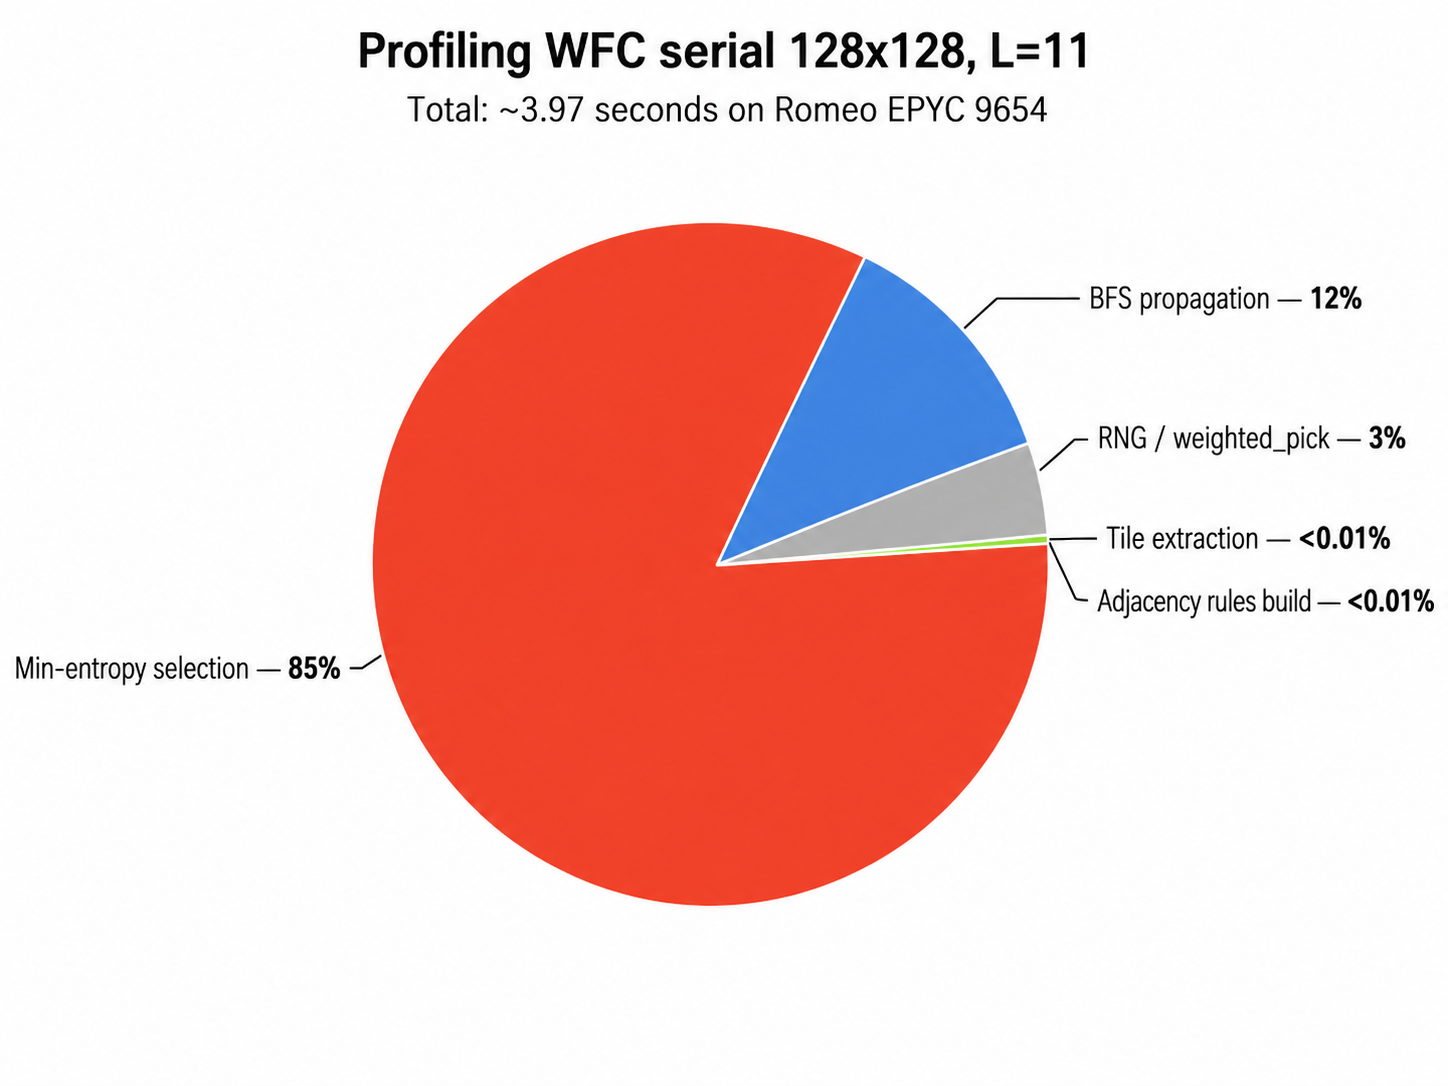
\includegraphics[width=0.7\linewidth]{results/figures/schemas/profile_breakdown.png}
\caption{Décomposition du temps sur 128×128 binaire. La sélection min-entropie domine.}
\label{fig:profile_breakdown}
\end{figure}

\subsection{Temps absolus de référence}

\begin{table}[H]
\centering
\begin{tabular}{lrr}
\toprule
\textbf{Taille} & \textbf{Solve serial (s)} & \textbf{Throughput (Mcells/s)} \\
\midrule
32×32 & 0.015 & 68 \\
64×64 & 0.247 & 16.6 \\
128×128 & 3.97 & 4.13 \\
256×256 & 61.4 & 1.07 \\
\bottomrule
\end{tabular}
\caption{Performance séquentielle sur Romeo, sample binary\_L11. Le throughput chute avec la taille à cause des cache misses (la wave déborde de la L2 à 256×256).}
\label{tab:res:serial}
\end{table}

% =============================================================================
\section{Scaling OpenMP : strong scaling}
\label{sec:res:omp_scaling}
% =============================================================================

\subsection{Speedup binary\_L11 sur Romeo}

La courbe de speedup (Fig.~\ref{fig:speedup_binary}) trace $S(p)$ pour les quatre tailles testées. Toutes les courbes montent jusqu'à un peak situé entre 4 et 16 threads selon la taille, puis chutent : à 256$\times$256, peak 8.23$\times$ à 16 threads ; à 32$\times$32, on n'atteint jamais 1.2$\times$. La forme générale est bien celle prédite par Amdahl complétée par des coûts \emph{supra}-Amdahl (fork/join, contention, frontières BFS) qui dominent au-delà du peak.

\begin{figure}[H]
\centering

\includegraphics[width=0.85\linewidth]{results/figures/scaling/speedup_binary_L11.png}
\caption{Speedup binary\_L11. Plus la grille est grande, plus le peak est élevé et plus il se déplace vers la droite.}
\label{fig:speedup_binary}
\end{figure}

La bande min/max (Fig.~\ref{fig:speedup_band_binary}) quantifie la variance entre les 3 répétitions de chaque configuration. Lecture pratique : entre 1 et 8 threads, la bande est étroite (régime stable, mesures reproductibles) ; au-delà de 32 threads, la bande s'élargit fortement, les régressions exactes varient d'un run à l'autre.

\begin{figure}[H]
\centering

\includegraphics[width=0.85\linewidth]{results/figures/scaling/speedup_band_binary_L11.png}
\caption{Bande min/max binary\_L11 (3 répétitions). Étroite en régime stable (1-8 threads), large au-delà de 32 threads.}
\label{fig:speedup_band_binary}
\end{figure}

L'efficacité parallèle $E(p) = S(p)/p$ (Fig.~\ref{fig:efficiency_binary}) donne une lecture normalisée : à 16 threads sur 256$\times$256 nous sommes à $E = 0.51$ (51\% d'efficacité) ; au-delà de 32 threads, $E$ chute sous 0.1 sur toutes les tailles. Cela quantifie un point important : ce n'est pas un \emph{plateau}, c'est un \emph{décrochage} brutal causé par la barrière par niveau BFS.

\begin{figure}[H]
\centering

\includegraphics[width=0.85\linewidth]{results/figures/scaling/efficiency_binary_L11.png}
\caption{Efficacité parallèle binary\_L11. Décrochage net au-delà de 32 threads, pas un plateau.}
\label{fig:efficiency_binary}
\end{figure}

Le throughput (Fig.~\ref{fig:throughput_binary}) inverse la lecture : à taille fixée, l'amortissement parallèle paie quand la grille est grande. Le pic à 15.4 Mcells/s sur 256$\times$256, 16 threads, est $14\times$ supérieur au serial sur la même taille (1.07 Mcells/s, Tab.~\ref{tab:res:serial}). Cela vient en partie du parallélisme et en partie du masquage des latences mémoire (la wave 524 KB déborde de la L2, le parallélisme aide à amortir les latences).

\begin{figure}[H]
\centering
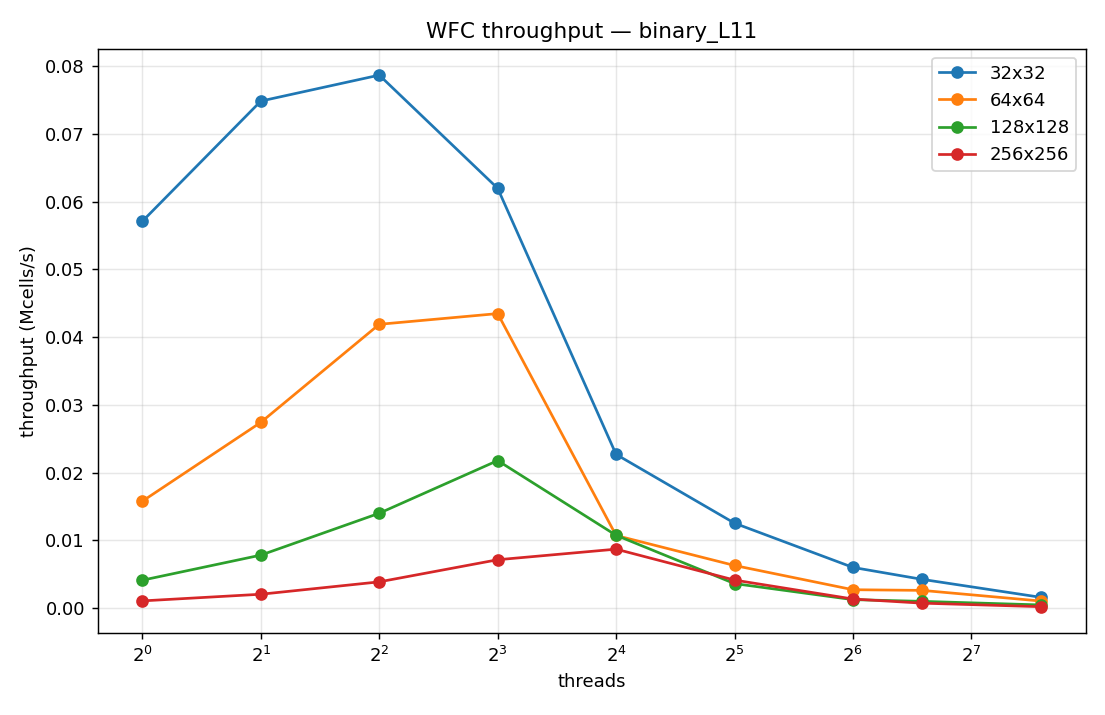
\includegraphics[width=0.85\linewidth]{results/figures/scaling/throughput_binary_L11.png}
\caption{Throughput binary\_L11. Pic 15.4 Mcells/s à 16 threads sur 256$\times$256 ($14\times$ vs serial).}
\label{fig:throughput_binary}
\end{figure}

Le heatmap taille$\times$threads (Fig.~\ref{fig:heatmap_binary}) résume le tout en deux dimensions : la \emph{diagonale} verte (sweet spot) montre que la taille optimale de grille \emph{suit} le nombre de threads. Lecture directe : à 8 threads, optimum vers 128$\times$128 ; à 16 threads, optimum vers 256$\times$256 ; à 32+ threads, le sweet spot sort de la zone mesurée (les runs 512$\times$512 ont timeout à 4h sur Romeo).

\begin{figure}[H]
\centering

\includegraphics[width=0.85\linewidth]{results/figures/scaling/heatmap_binary_L11.png}
\caption{Heatmap binary\_L11 (taille $\times$ threads, couleur = temps). Le sweet spot diagonal indique que la taille optimale suit le nombre de threads.}
\label{fig:heatmap_binary}
\end{figure}

\begin{table}[H]
\centering
\begin{tabular}{lrrrrrrrr}
\toprule
\textbf{Taille} & \textbf{1t} & \textbf{2t} & \textbf{4t} & \textbf{8t} & \textbf{16t} & \textbf{32t} & \textbf{64t} & \textbf{192t} \\
\midrule
32×32 & 1.00× & 1.10× & 1.16× & 0.91× & 0.33× & 0.18× & 0.09× & 0.02× \\
64×64 & 0.96× & 1.66× & 2.54× & 2.64× & 0.65× & 0.38× & 0.16× & 0.06× \\
128×128 & 1.00× & 1.89× & 3.39× & 5.27× & 2.60× & 0.87× & 0.30× & 0.11× \\
\textbf{256×256} & \textbf{1.00×} & \textbf{1.93×} & \textbf{3.65×} & \textbf{6.73×} & \textbf{8.23×} & \textbf{3.91×} & \textbf{1.26×} & \textbf{0.19×} \\
\bottomrule
\end{tabular}
\caption{Strong scaling binary\_L11 sur Romeo (job 543692). Peak 8.23× à 16 threads sur 256×256. Régression brutale au-delà du peak.}
\label{tab:res:speedup_binary}
\end{table}

\begin{important}{Lecture du tableau}
\begin{itemize}
    \item À 32×32, le parallélisme ne paie jamais : la grille est trop petite pour amortir le coût des tasks.
    \item À 64×64, peak modeste à 4-8 threads ; au-delà, régression rapide.
    \item À 128×128, peak 5.27× à 8 threads, déjà honorable.
    \item À 256×256, peak 8.23× à 16 threads (51\% d'efficacité parallèle). C'est notre meilleur résultat.
    \item Au-delà du peak (32+ threads), régression brutale jusqu'à 0.02× la baseline à 192 threads sur 32×32 (le solver tourne 50× plus lentement que le serial).
\end{itemize}
\end{important}

\subsection{Causes de la régression à haut nombre de threads}

Trois causes dominent :

\begin{enumerate}
    \item \textbf{Frontière BFS trop courte} : un niveau de 10 cellules sur 192 threads → 18 threads sur 19 attendent à la barrière. Le coût synchronisation domine.

    \item \textbf{Fork/join répété} : la barrière par niveau coûte $\sim 50$ µs sur 192 cores. Pour 8000 niveaux : 400 ms incompressibles, à comparer aux $\sim 100$ ms de travail utile.

    \item \textbf{Contention atomique inter-NUMA} : \texttt{\_\_atomic\_fetch\_and} cross-NUMA = ping-pong de cache lines à 1-3 µs par opération.
\end{enumerate}

L'optim « frontier-threshold » (Section~\ref{sec:res:optim_frontier}) atténue (1) et (2) mais pas (3).

% =============================================================================
\section{Modèle d'Amdahl}
\label{sec:res:amdahl}
% =============================================================================

Pour caractériser le scaling, nous fittons Amdahl $S(p) = 1 / ((1-f) + f/p)$ par moindres carrés non-linéaires sur la portion croissante de chaque courbe (avant le décrochage). Le fit retourne $f$ (fraction parallélisable) et le ceiling théorique $S_\infty = 1/(1-f)$. Les courbes sont en échelle log-log avec la droite « idéale » $S = p$ pour repère.

\subsection{Évolution du fit avec la taille de grille}

La mosaïque (Fig.~\ref{fig:amdahl_binary_grid}) trace les 4 fits binary\_L11 pour les 4 tailles testées. La fraction parallélisable $f$ croît brutalement avec la taille : 0.18 (32$\times$32) $\to$ 0.74 (64$\times$64) $\to$ 0.93 (128$\times$128) $\to$ 0.94 (256$\times$256). Lecture algorithmique : les coûts fixes (extraction tuiles, init wave, fork/join initial) deviennent rapidement négligeables face au travail utile dès que la grille dépasse 64$\times$64.

\begin{figure}[H]
\centering
\begin{subfigure}[t]{0.48\linewidth}
\centering
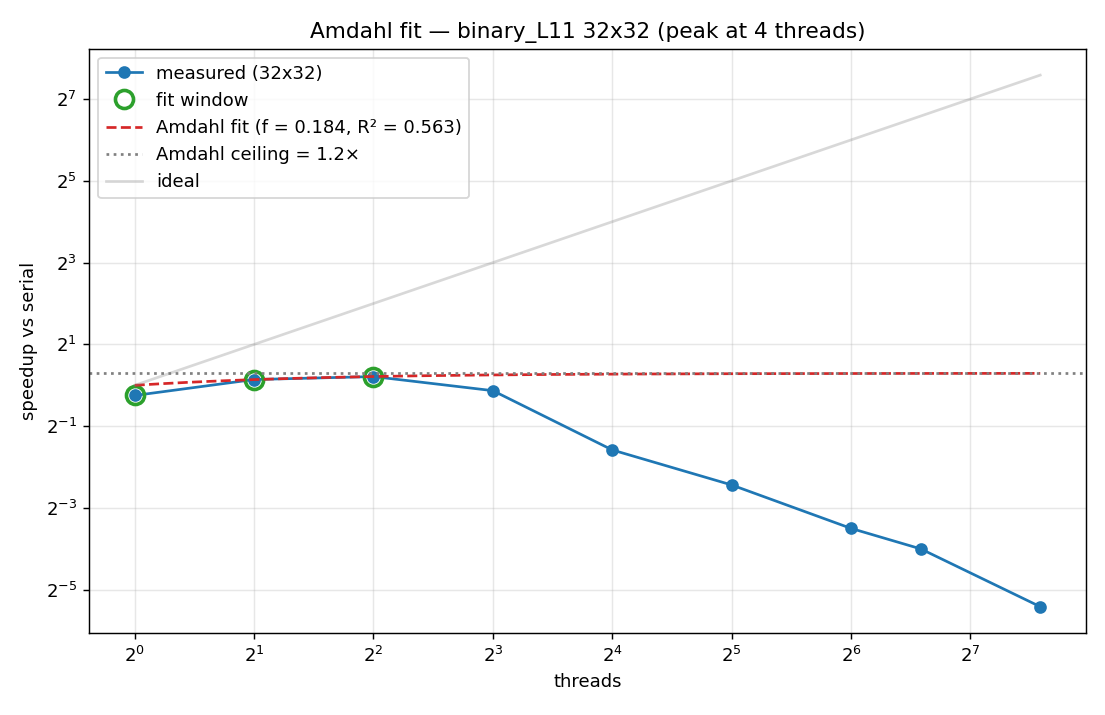
\includegraphics[width=\linewidth]{results/figures/amdahl/amdahl_binary_L11_32.png}
\caption{32×32, $f = 0.18$, ceiling $1.2\times$.}
\end{subfigure}\hfill
\begin{subfigure}[t]{0.48\linewidth}
\centering
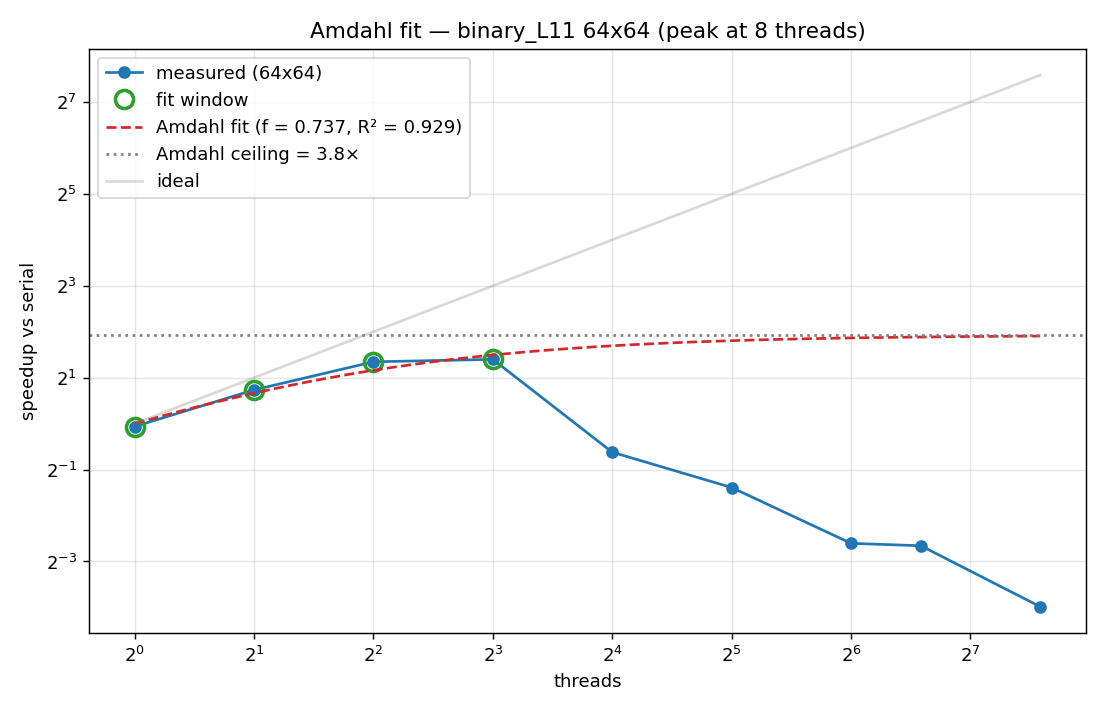
\includegraphics[width=\linewidth]{results/figures/amdahl/amdahl_binary_L11_64.png}
\caption{64×64, $f = 0.74$, ceiling $3.8\times$.}
\end{subfigure}

\vspace{0.5em}

\begin{subfigure}[t]{0.48\linewidth}
\centering
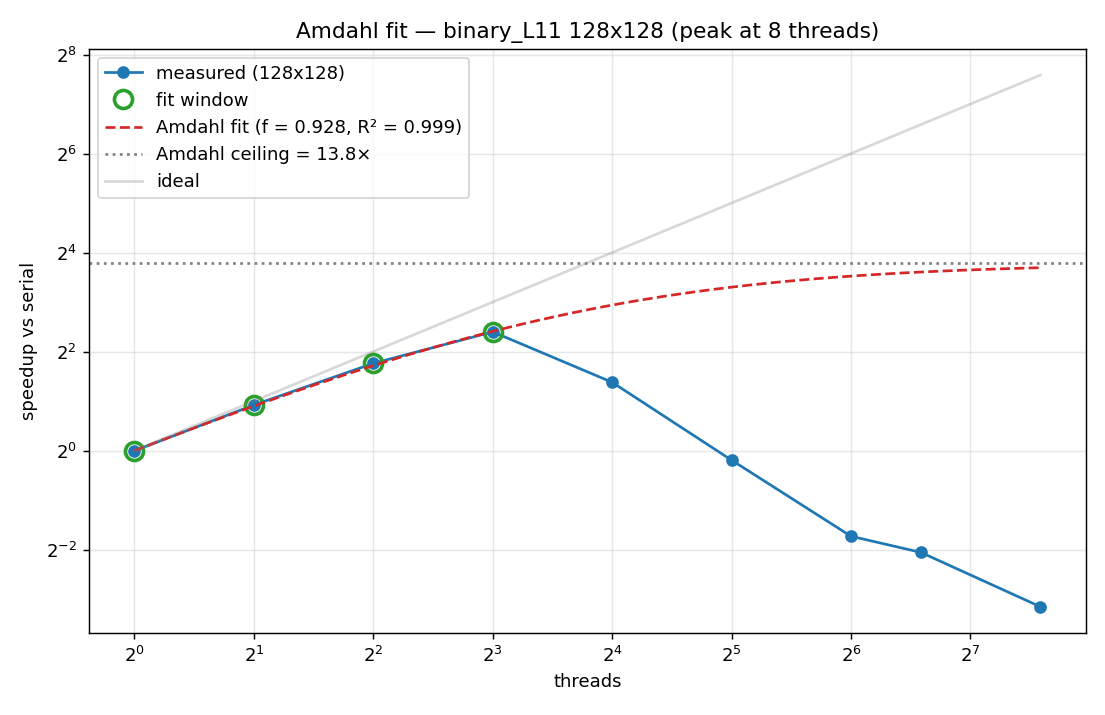
\includegraphics[width=\linewidth]{results/figures/amdahl/amdahl_binary_L11_128.png}
\caption{128×128, $f = 0.93$, ceiling $13.8\times$.}
\end{subfigure}\hfill
\begin{subfigure}[t]{0.48\linewidth}
\centering
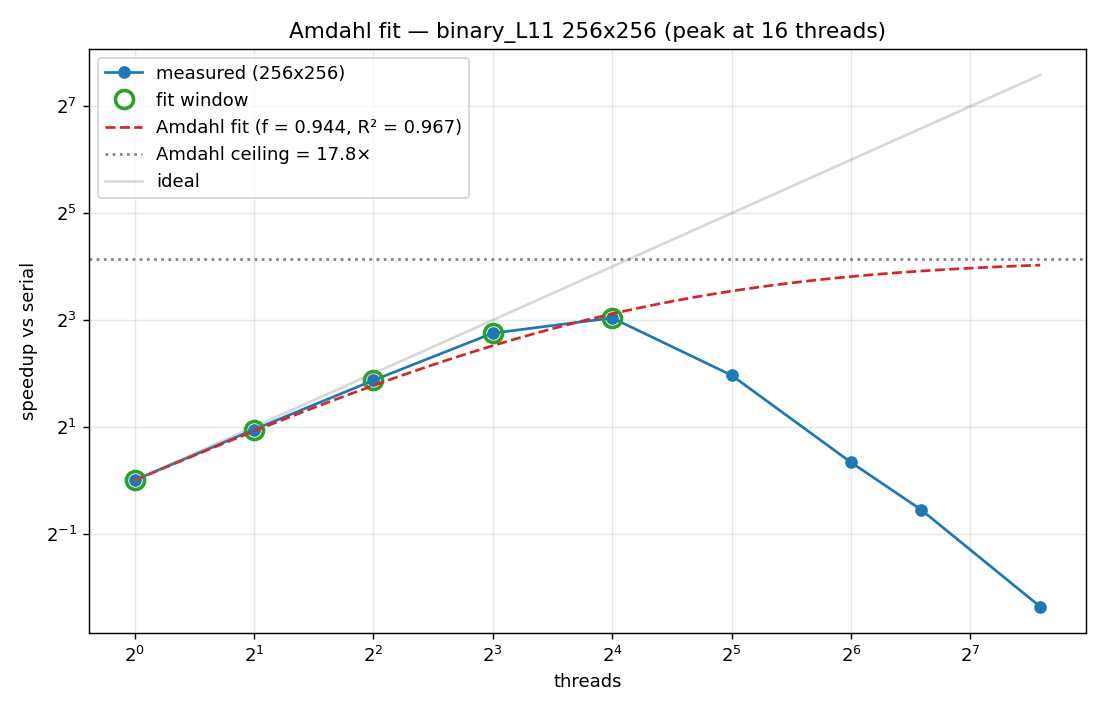
\includegraphics[width=\linewidth]{results/figures/amdahl/amdahl_binary_L11_256.png}
\caption{256×256, $f = 0.94$, ceiling $17.8\times$.}
\end{subfigure}

\caption[Évolution du fit Amdahl binary\_L11 par taille.]{Évolution
du fit Amdahl binary\_L11 avec la taille de grille. La fraction
parallélisable $f$ croît rapidement de 0.18 (32×32) à 0.94 (256×256) :
plus la grille est grande, plus propagation et sélection min-entropie
dominent face aux coûts fixes.}
\label{fig:amdahl_binary_grid}
\end{figure}

\subsection{Effet de l'optim « frontier-threshold » sur Amdahl}

Re-fitter Amdahl après activation de l'optim frontier-threshold (Fig.~\ref{fig:amdahl_binary_optim}) déplace les paramètres du modèle : $f$ passe de 0.928 à 0.956, le ceiling théorique de $13.8\times$ à $22.9\times$. Le peak observé monte de $5.27\times$ à $6.10\times$ : l'optim ne ferme pas l'écart au ceiling (les coûts supra-Amdahl restent), mais elle pousse le mur plus loin.

\begin{figure}[H]
\centering
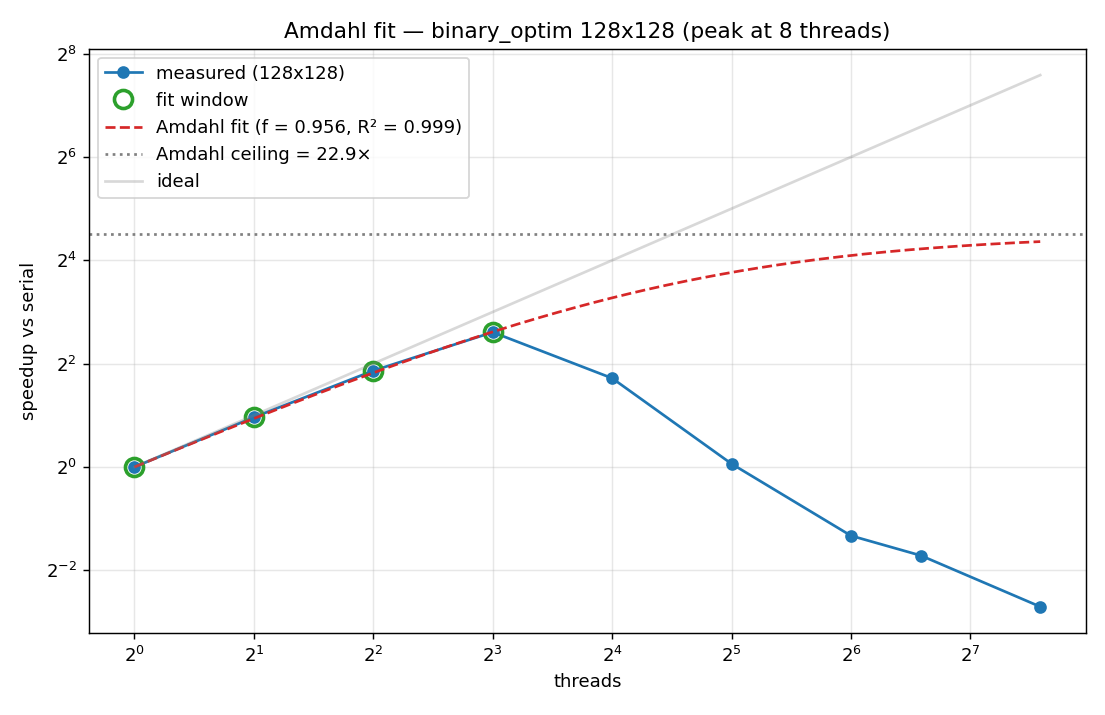
\includegraphics[width=0.85\linewidth]{results/figures/amdahl/amdahl_binary_optim_128.png}
\caption[Fit Amdahl binary 128 après optim frontier-threshold.]{Fit
Amdahl binary\_L11 128×128 après frontier-threshold. $f$ passe de
0.928 à 0.956, ceiling de $13.8\times$ à $22.9\times$.}
\label{fig:amdahl_binary_optim}
\end{figure}

\subsection{Amdahl sur autres samples}

La mosaïque par sample (Fig.~\ref{fig:amdahl_other_samples}) compare terrain\_L33 et smooth\_N3 sur 3 tailles. terrain\_L33 suit le même pattern que binary\_L11 (croissance régulière de $f$ avec la taille). smooth\_N3 plafonne à $f = 0.74$ même à 128$\times$128 : peu de tuiles ($L=12$) combiné à $N=3$ produit des frontières BFS courtes qui propagent peu, donc peu de parallélisme exploitable. C'est une limite \emph{structurelle} du sample, pas une marge d'optimisation.

\begin{figure}[H]
\centering
\begin{subfigure}[t]{0.31\linewidth}
\centering
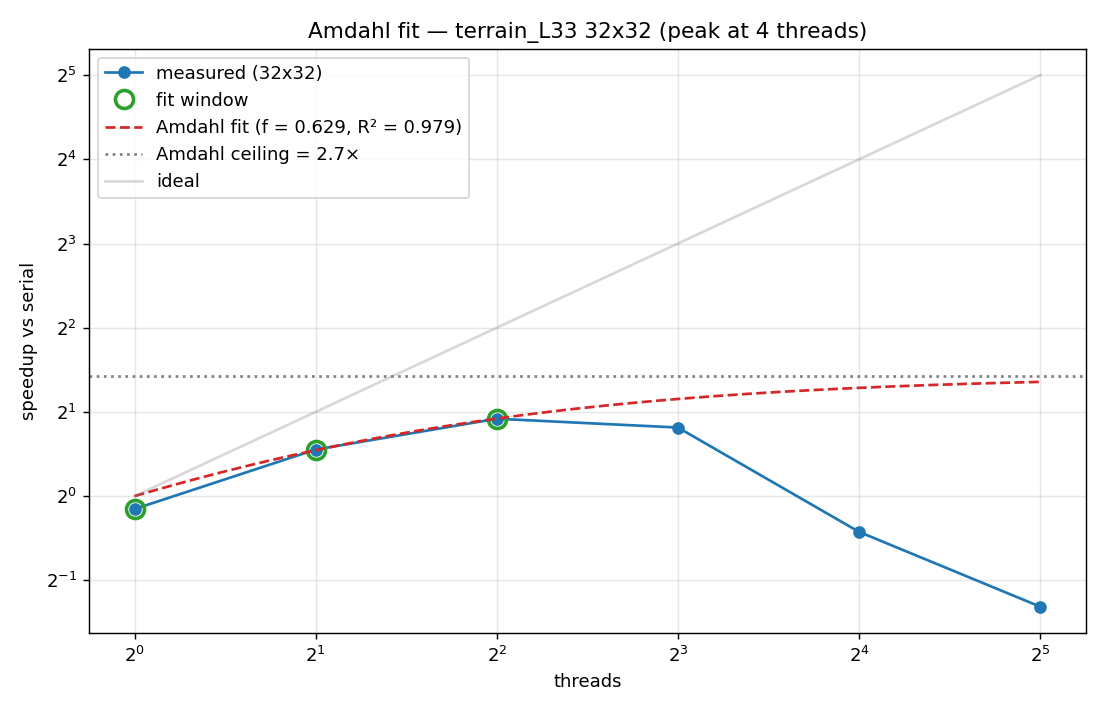
\includegraphics[width=\linewidth]{results/figures/amdahl/amdahl_terrain_L33_32.png}
\caption{terrain 32×32.}
\end{subfigure}\hfill
\begin{subfigure}[t]{0.31\linewidth}
\centering
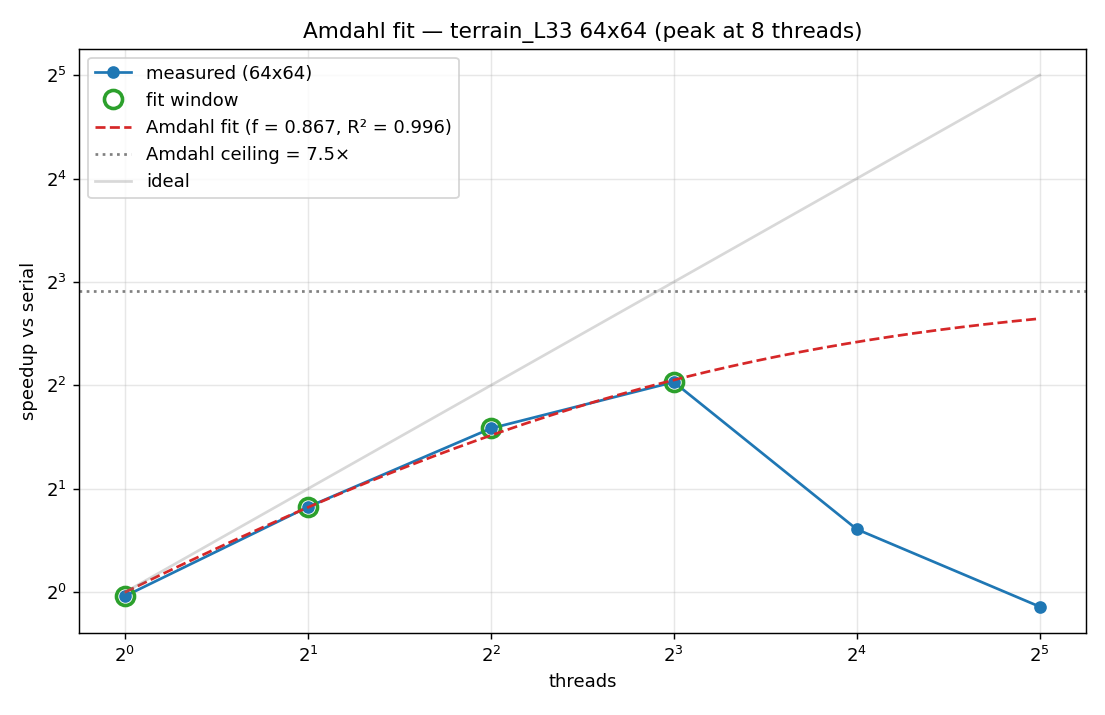
\includegraphics[width=\linewidth]{results/figures/amdahl/amdahl_terrain_L33_64.png}
\caption{terrain 64×64.}
\end{subfigure}\hfill
\begin{subfigure}[t]{0.31\linewidth}
\centering
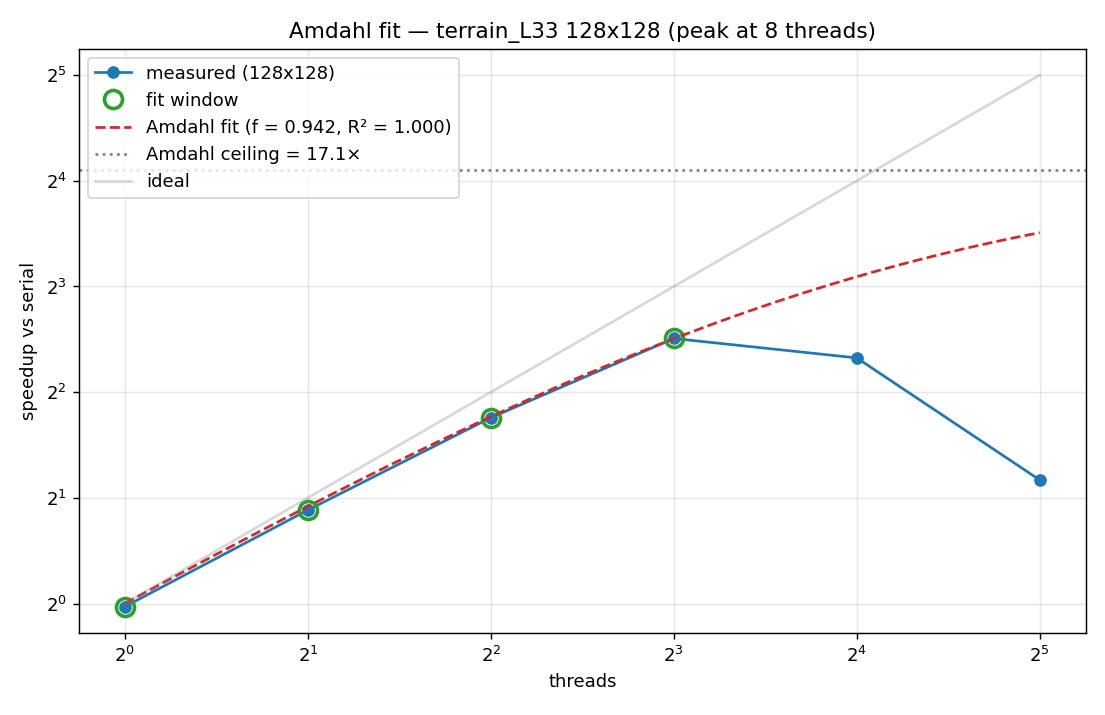
\includegraphics[width=\linewidth]{results/figures/amdahl/amdahl_terrain_L33_128.png}
\caption{terrain 128×128, $f=0.94$.}
\end{subfigure}

\vspace{0.5em}

\begin{subfigure}[t]{0.31\linewidth}
\centering
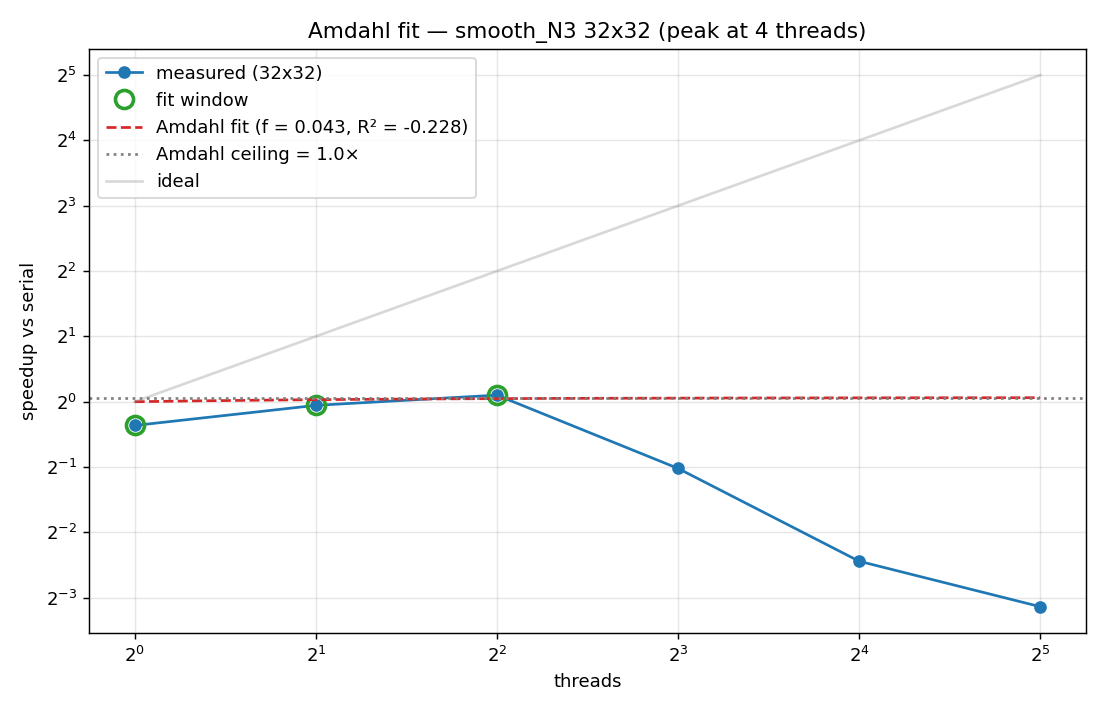
\includegraphics[width=\linewidth]{results/figures/amdahl/amdahl_smooth_N3_32.png}
\caption{smooth\_N3 32×32.}
\end{subfigure}\hfill
\begin{subfigure}[t]{0.31\linewidth}
\centering
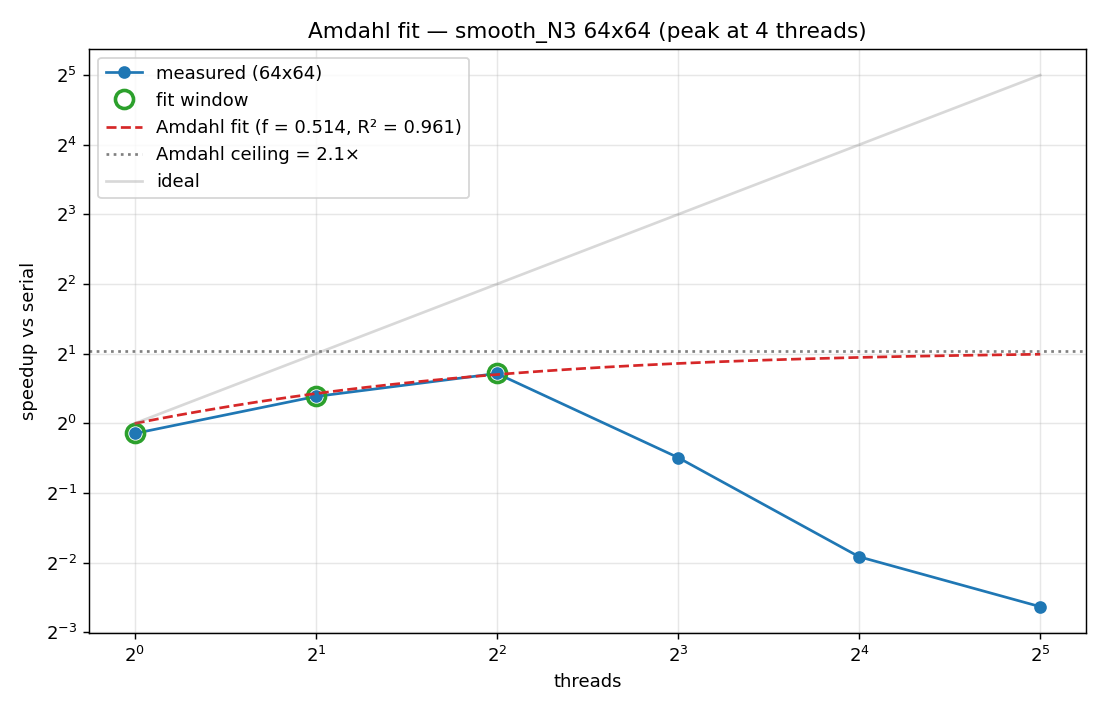
\includegraphics[width=\linewidth]{results/figures/amdahl/amdahl_smooth_N3_64.png}
\caption{smooth\_N3 64×64.}
\end{subfigure}\hfill
\begin{subfigure}[t]{0.31\linewidth}
\centering
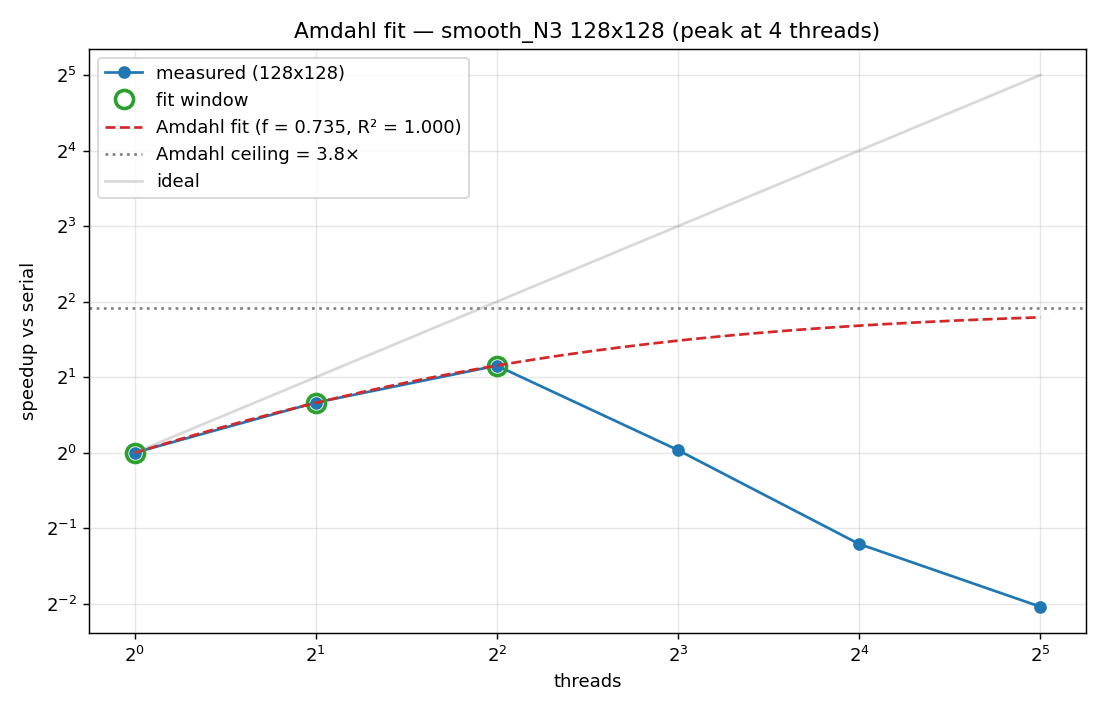
\includegraphics[width=\linewidth]{results/figures/amdahl/amdahl_smooth_N3_128.png}
\caption{smooth\_N3 128×128, $f=0.74$.}
\end{subfigure}

\caption[Fits Amdahl par sample : terrain et smooth.]{Fits Amdahl
par sample × taille. terrain\_L33 suit le même pattern que
binary\_L11 (croissance de $f$ avec la taille). smooth\_N3 plafonne à
$f = 0.74$ même à 128×128 : peu de tuiles ($L=12$) et $N=3$ $\to$
parallélisme structurel limité, indépendamment de la grille.}
\label{fig:amdahl_other_samples}
\end{figure}

\begin{table}[H]
\centering
\begin{tabular}{llrrrrr}
\toprule
\textbf{Label} & \textbf{Size} & \textbf{$f$} & \textbf{$R^2$} & \textbf{Ceiling} & \textbf{Peak} & \textbf{Ratio} \\
\midrule
binary\_L11 & 32 & 0.184 & 0.563 & 1.2× & 1.16× & 95\% \\
binary\_L11 & 64 & 0.737 & 0.929 & 3.8× & 2.64× & 69\% \\
binary\_L11 & 128 & 0.928 & 0.999 & 13.8× & 5.27× & 38\% \\
binary\_L11 & 256 & 0.944 & 0.967 & 17.8× & 8.23× & 46\% \\
binary\_optim & 128 & 0.956 & 0.999 & 22.9× & 6.10× & 27\% \\
terrain\_L33 & 64 & 0.867 & 0.996 & 7.5× & 4.09× & 54\% \\
terrain\_L33 & 128 & 0.942 & 1.000 & 17.1× & 5.69× & 33\% \\
smooth\_N3 & 128 & 0.735 & 1.000 & 3.8× & 2.23× & 59\% \\
\bottomrule
\end{tabular}
\caption{Fits Amdahl par configuration. À 128 et 256, $f \approx 0.94$ pour binary et terrain : le code est ~94\% parallélisable, ceiling théorique 14-18×. Le peak observé reste à 33-46\% du ceiling : Amdahl suppose un parallélisme parfait, la réalité inclut des coûts supra-linéaires.}
\label{tab:res:amdahl}
\end{table}

\begin{important}{Lecture du fit Amdahl}
\begin{itemize}
    \item L'optim « frontier-threshold » pousse $f$ de 0.928 à 0.956 sur 128×128 (peak 5.27× → 6.10×, ceiling théorique 13.8 → 22.9).
    \item Le ratio peak/ceiling baisse, mais le peak absolu monte. L'optim aide.
    \item \texttt{smooth\_N3} a $f = 0.735$ au max, beaucoup moins parallélisable. Cause : peu de tuiles ($L=12$) + $N=3$ = peu de parallélisme par cellule (analyse en Section~\ref{sec:res:varying_datasets}).
\end{itemize}
\end{important}

% =============================================================================
\section{Varying datasets : impact du sample}
\label{sec:res:varying_datasets}
% =============================================================================

À taille de grille fixée (128×128) et thread count variable, le sample modifie significativement le scaling.

\subsection{terrain\_L33 vs binary\_L11}

terrain\_L33 (33 tuiles, $N=2$) scale mieux que binary\_L11 à taille égale. Sur 128$\times$128 (Fig.~\ref{fig:speedup_terrain}), le peak est 5.69$\times$ à 8 threads contre 5.27$\times$ pour binary\_L11. La différence vient du travail par cellule : 33 bits à manipuler par cellule vs 11, donc plus d'opérations utiles à amortir, et l'overhead OMP relatif diminue.

\begin{figure}[H]
\centering
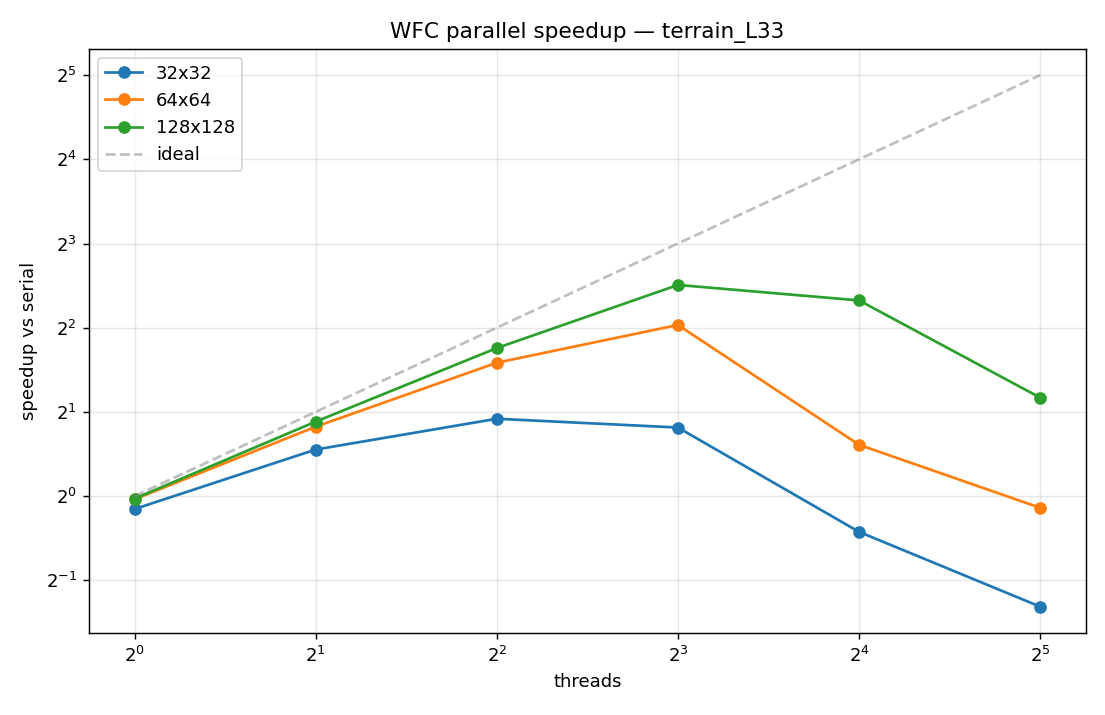
\includegraphics[width=0.85\linewidth]{results/figures/scaling/speedup_terrain_L33.png}
\caption{Speedup terrain\_L33. Peak 5.69$\times$ à 8 threads sur 128$\times$128.}
\label{fig:speedup_terrain}
\end{figure}

L'efficacité et le throughput (Fig.~\ref{fig:scaling_terrain_combo}) confirment : à 8 threads sur 128$\times$128, $E \approx 0.71$ (71\% d'efficacité, vs 65\% pour binary à la même configuration). Le décrochage post-peak est aussi moins brutal, la bande min/max (Fig.~\ref{fig:speedup_band_terrain}) reste étroite jusqu'à 16 threads.

\begin{figure}[H]
\centering
\begin{subfigure}[t]{0.48\linewidth}
\centering
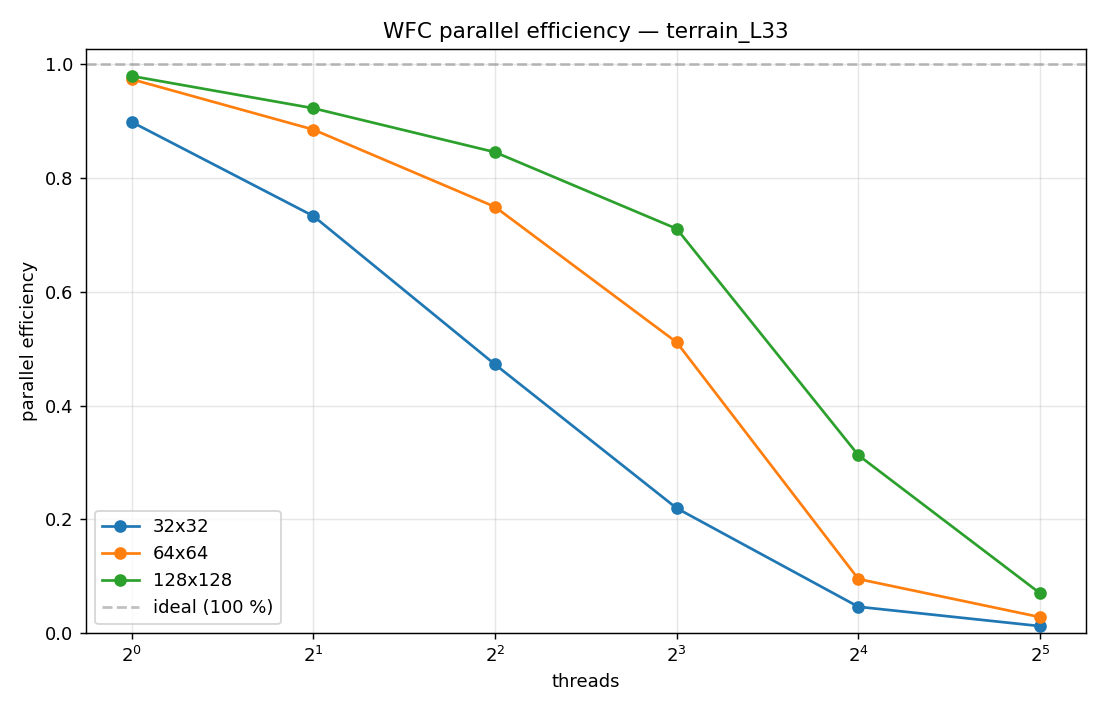
\includegraphics[width=\linewidth]{results/figures/scaling/efficiency_terrain_L33.png}
\caption{Efficacité parallèle terrain\_L33.}
\end{subfigure}\hfill
\begin{subfigure}[t]{0.48\linewidth}
\centering
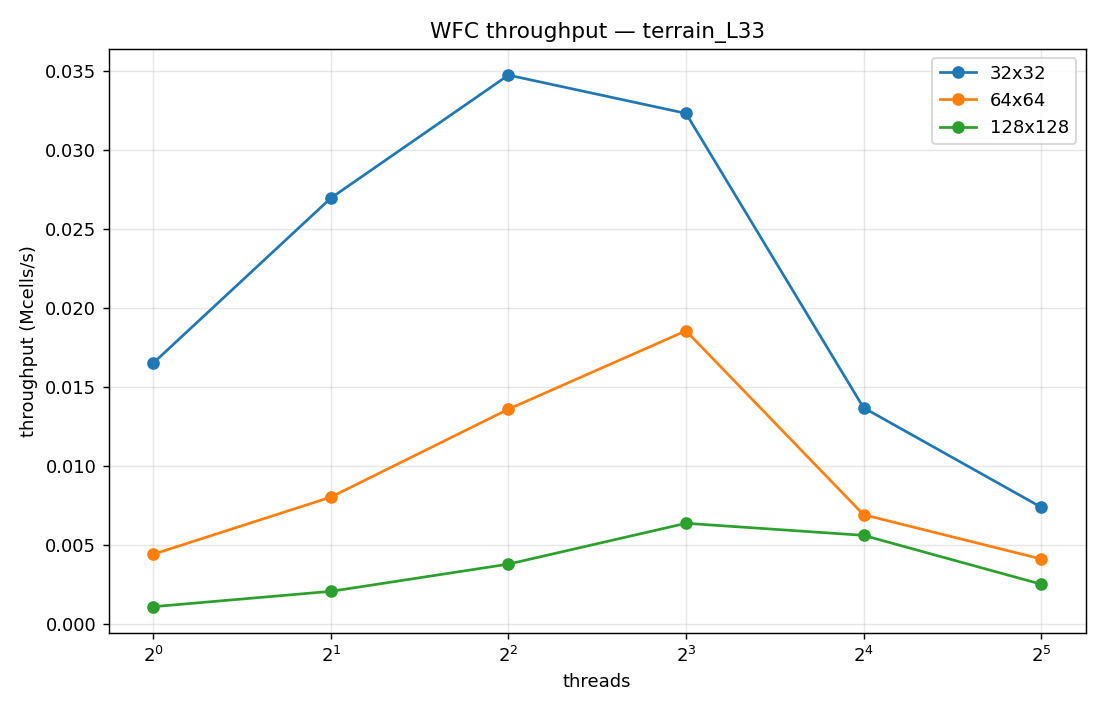
\includegraphics[width=\linewidth]{results/figures/scaling/throughput_terrain_L33.png}
\caption{Throughput terrain\_L33.}
\end{subfigure}

\caption{terrain\_L33 efficacité + throughput. À 128$\times$128 et 8 threads, $E \approx 0.71$ (vs 0.65 pour binary\_L11).}
\label{fig:scaling_terrain_combo}
\end{figure}

Le heatmap terrain\_L33 (Fig.~\ref{fig:heatmap_terrain}) montre un sweet spot diagonal plus large que pour binary\_L11 : la plage de configurations exploitables est plus tolérante au choix taille$\times$threads.

\begin{figure}[H]
\centering
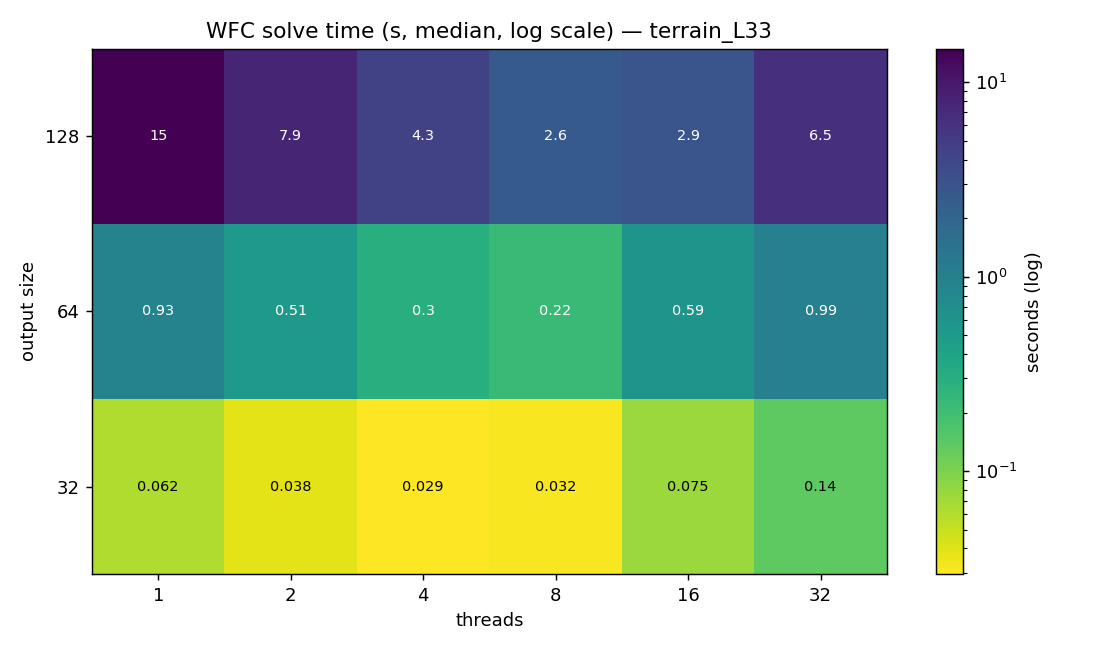
\includegraphics[width=0.85\linewidth]{results/figures/scaling/heatmap_terrain_L33.png}
\caption{Heatmap terrain\_L33. Sweet spot diagonal plus large que binary\_L11.}
\label{fig:heatmap_terrain}
\end{figure}

\begin{figure}[H]
\centering
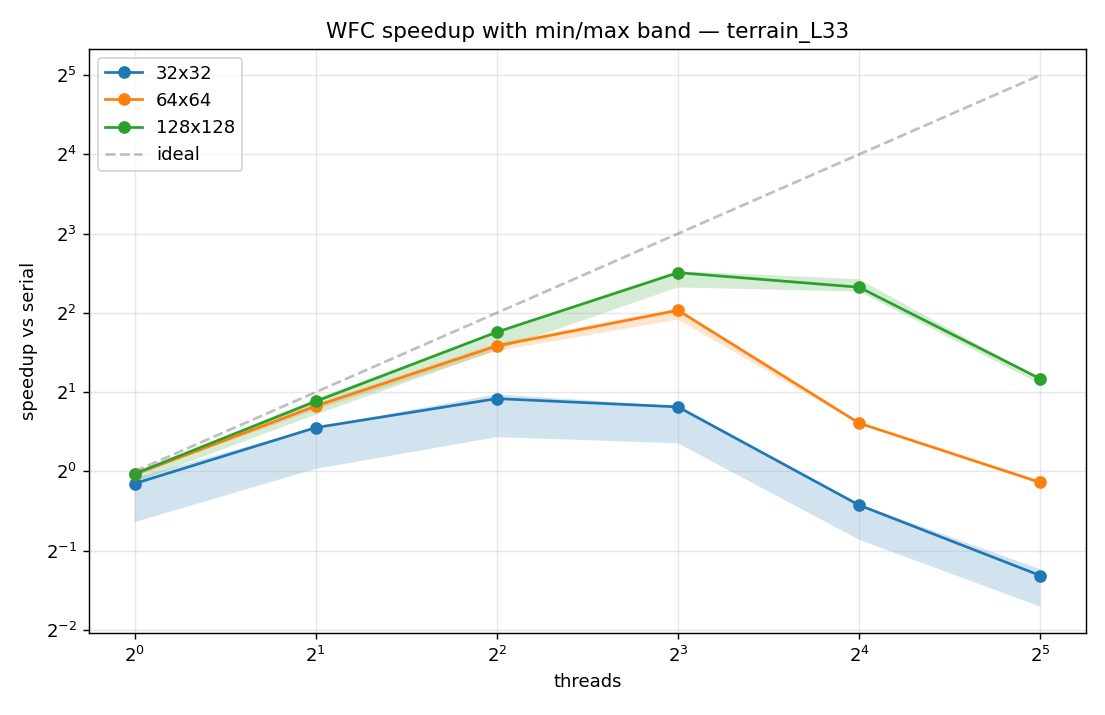
\includegraphics[width=0.85\linewidth]{results/figures/scaling/speedup_band_terrain_L33.png}
\caption{Bande min/max terrain\_L33. Étroite jusqu'à 16 threads.}
\label{fig:speedup_band_terrain}
\end{figure}

\begin{table}[H]
\centering
\begin{tabular}{lrrrrrr}
\toprule
\textbf{Sample} & \textbf{$L$} & \textbf{1t} & \textbf{4t} & \textbf{8t} & \textbf{16t} & \textbf{32t} \\
\midrule
binary\_L11 128×128 & 11 & 1.00× & 3.39× & 5.27× & 2.60× & 0.87× \\
terrain\_L33 128×128 & 33 & 1.00× & 3.43× & \textbf{5.69×} & 4.81× & 2.13× \\
\bottomrule
\end{tabular}
\caption{terrain\_L33 (33 tuiles) atteint un meilleur peak que binary\_L11 (11 tuiles) à taille égale. La différence vient du travail par cellule : plus de bits → meilleur amortissement OMP.}
\label{tab:res:terrain_vs_binary}
\end{table}

\subsection{smooth\_N3, le cas pathologique}

smooth\_N3 (12 tuiles, $N=3$, gradients lisses) plafonne à 2.23$\times$ à 4 threads sur 128$\times$128 (Fig.~\ref{fig:speedup_smooth}) et régresse dès 8 threads. Cause : les motifs lisses produisent des frontières BFS très courtes (peu de cellules touchées par niveau). Combiné à 12 tuiles seulement, le travail par niveau est insuffisant pour amortir les barrières OMP au-delà de 4 threads.

\begin{figure}[H]
\centering

\includegraphics[width=0.85\linewidth]{results/figures/scaling/speedup_smooth_N3.png}
\caption{Speedup smooth\_N3. Peak 2.23$\times$ à 4 threads, régression dès 8.}
\label{fig:speedup_smooth}
\end{figure}

L'efficacité et le throughput (Fig.~\ref{fig:scaling_smooth_combo}) confirment : plateau à 4 threads, puis décrochage. Le heatmap (Fig.~\ref{fig:heatmap_smooth}) montre un sweet spot étroit autour de 4 threads, indépendant de la taille de grille — c'est une borne \emph{structurelle} du sample, pas un paramètre à optimiser.

\begin{figure}[H]
\centering
\begin{subfigure}[t]{0.48\linewidth}
\centering

\includegraphics[width=\linewidth]{results/figures/scaling/efficiency_smooth_N3.png}
\caption{Efficacité smooth\_N3.}
\end{subfigure}\hfill
\begin{subfigure}[t]{0.48\linewidth}
\centering
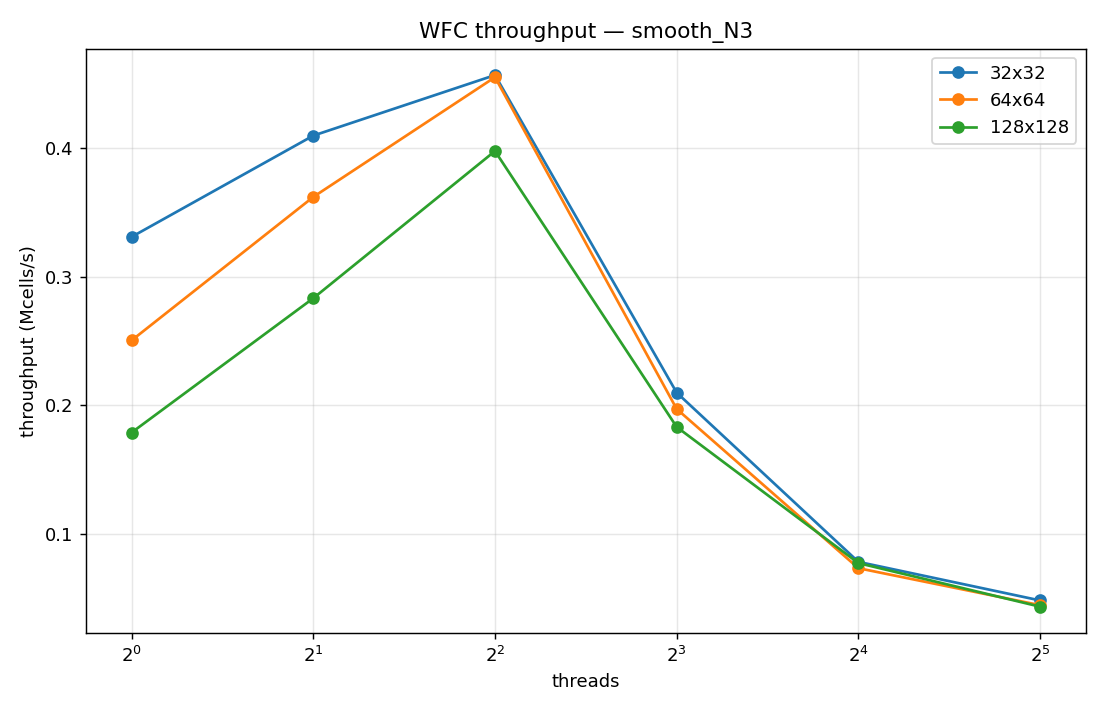
\includegraphics[width=\linewidth]{results/figures/scaling/throughput_smooth_N3.png}
\caption{Throughput smooth\_N3.}
\end{subfigure}

\caption{smooth\_N3 efficacité + throughput. Plateau à 4 threads, décrochage au-delà.}
\label{fig:scaling_smooth_combo}
\end{figure}

\begin{figure}[H]
\centering

\includegraphics[width=0.85\linewidth]{results/figures/scaling/heatmap_smooth_N3.png}
\caption{Heatmap smooth\_N3. Sweet spot étroit autour de 4 threads, indépendant de la taille.}
\label{fig:heatmap_smooth}
\end{figure}

\begin{figure}[H]
\centering

\includegraphics[width=0.85\linewidth]{results/figures/scaling/speedup_band_smooth_N3.png}
\caption{Bande min/max smooth\_N3. Élargissement dès 8 threads : variance forte hors du sweet spot.}
\label{fig:speedup_band_smooth}
\end{figure}

\begin{table}[H]
\centering
\begin{tabular}{lrrrrrr}
\toprule
\textbf{Taille} & \textbf{1t} & \textbf{2t} & \textbf{4t} & \textbf{8t} & \textbf{16t} & \textbf{32t} \\
\midrule
32×32 & 1.00× & 0.96× & 1.07× & 0.49× & 0.18× & 0.11× \\
64×64 & 1.00× & 1.50× & 1.64× & 0.71× & 0.27× & 0.16× \\
128×128 & 1.00× & 1.85× & \textbf{2.23×} & 1.16× & 0.43× & 0.24× \\
\bottomrule
\end{tabular}
\caption{smooth\_N3 plafonne à 2.23×. Cause : $L = 12$ tuiles (peu) + $N = 3$ (offsets $5 \times 5 = 25$) → 300 ops/cell, à comparer à 99 pour binary. Frontières BFS courtes car les motifs lisses propagent peu.}
\label{tab:res:smooth_N3}
\end{table}

\begin{important}{Pourquoi smooth\_N3 plafonne}
\begin{itemize}
    \item Sample de 12 tuiles seulement (gradients lisses).
    \item $N = 3$ → offsets $5 \times 5 = 25$ vs 9 pour $N = 2$. Plus d'offsets, mais peu de bits par tuile à manipuler ($L = 12$ tient dans 1 mot).
    \item Motifs lisses → propagation locale qui modifie peu de cellules par niveau.
    \item Au total, chaque niveau BFS coûte trop peu pour amortir la barrière OMP au-delà de 4 threads.
\end{itemize}

Pas de fix algorithmique côté intra-attempt sans risquer de régresser binary. Contournements utilisateur : \texttt{--threads 4} (sweet spot intra-attempt) ou \texttt{--parallel-attempts K} si retries fréquents.
\end{important}

% =============================================================================
\section{Varying configurations : impact des paramètres}
\label{sec:res:varying_configs}
% =============================================================================

\subsection{Effet de la taille de grille}

À threads fixés (16) et sample fixé (binary\_L11) :

\begin{table}[H]
\centering
\begin{tabular}{lrrrr}
\toprule
\textbf{Taille} & \textbf{Wave size} & \textbf{Cache fit} & \textbf{Speedup 16t} & \textbf{Throughput (Mcells/s)} \\
\midrule
32×32 & 8 KB & L1 ✓ & 0.33× & 4.6 \\
64×64 & 32 KB & L1 borderline & 0.65× & 11.0 \\
128×128 & 128 KB & L2 ✓ & 2.60× & 13.4 \\
256×256 & 524 KB & L2 → LLC & 8.23× & \textbf{15.4} \\
\bottomrule
\end{tabular}
\caption{À 16 threads, le speedup et throughput augmentent avec la taille jusqu'à 256×256. La wave déborde de la L2 à 256×256 ; le parallélisme aide à amortir les latences mémoire.}
\label{tab:res:varying_size}
\end{table}

\subsection{Effet du paramètre $N$}

\begin{table}[H]
\centering
\begin{tabular}{lrrrr}
\toprule
\textbf{Sample} & \textbf{$N$} & \textbf{$L$} & \textbf{Solve serial 64×64 (s)} & \textbf{Note} \\
\midrule
\texttt{binary\_5x5} & 2 & 11 & 0.247 & Référence sujet \\
\texttt{multivalue\_terrain} & 2 & 33 & 0.520 & Plus de tuiles, plus lent \\
\texttt{multivalue\_terrain} & 3 & 73 & échec & $L = 73 > $ trop contraint \\
\texttt{multivalue\_smooth} & 3 & 12 & 0.020 & Sample petit, peu de tuiles \\
\bottomrule
\end{tabular}
\caption{Impact de $N$ et du sample sur le coût serial. $N = 3$ avec terrain échoue (trop contraint), $N = 2$ avec terrain converge en ~0.5 s.}
\label{tab:res:varying_N}
\end{table}

% =============================================================================
\section{Optim « frontier-threshold » : A/B Romeo}
\label{sec:res:optim_frontier}
% =============================================================================

\begin{figure}[H]
\centering
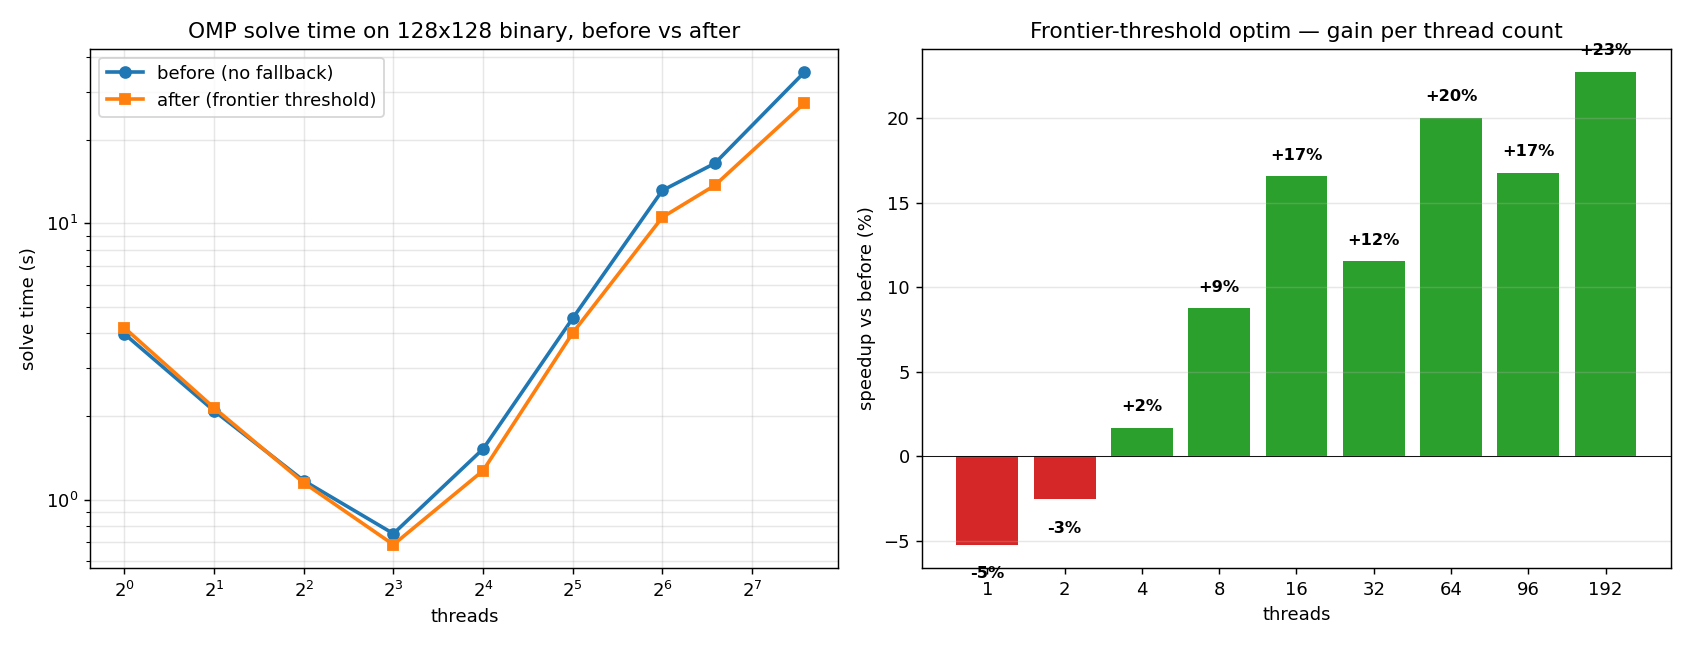
\includegraphics[width=0.85\linewidth]{results/figures/optim/frontier_threshold_compare.png}
\caption{A/B « frontier-threshold » sur binary\_L11 128×128 (job 544356).}
\label{fig:optim_frontier}
\end{figure}

\subsection{Profil de scaling complet \emph{après} optim (binary\_optim)}

Le run \texttt{binary\_optim} re-mesure binary\_L11 128×128 avec
\texttt{frontier-threshold} activé. On observe ainsi non pas un seul
nombre (gain à un thread count) mais l'évolution complète du
speedup, de l'efficacité et du throughput sous le régime optimisé.

\begin{figure}[H]
\centering
\begin{subfigure}[t]{0.48\linewidth}
\centering
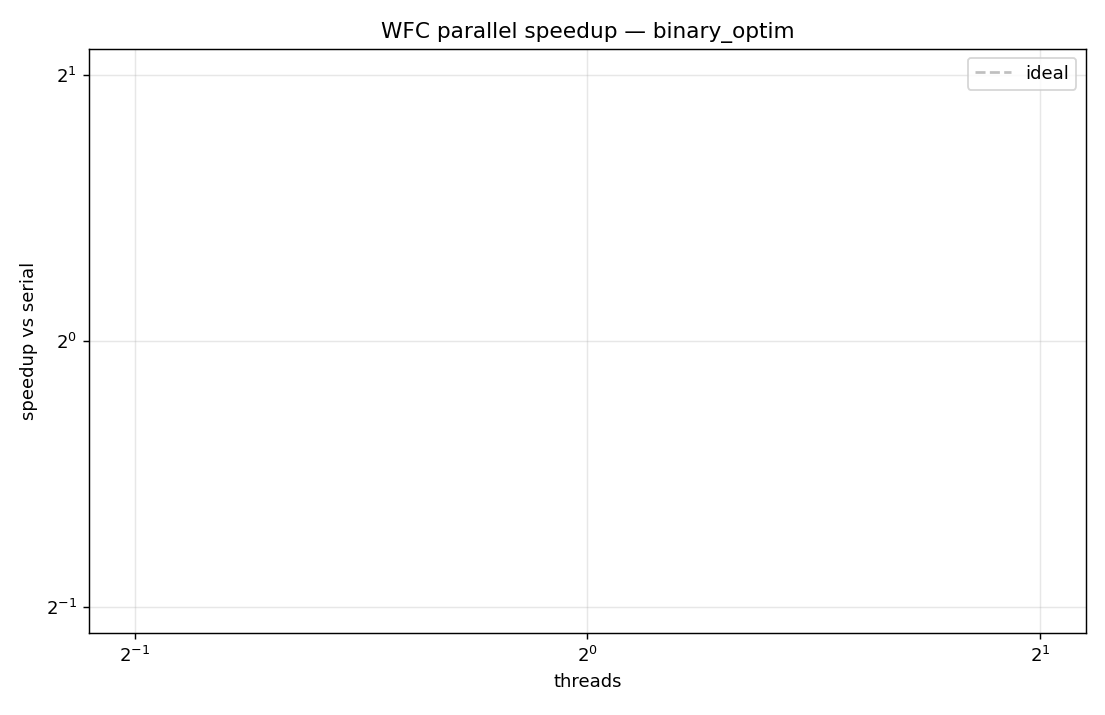
\includegraphics[width=\linewidth]{results/figures/scaling/speedup_binary_optim.png}
\caption{Speedup binary\_optim 128.}
\end{subfigure}\hfill
\begin{subfigure}[t]{0.48\linewidth}
\centering
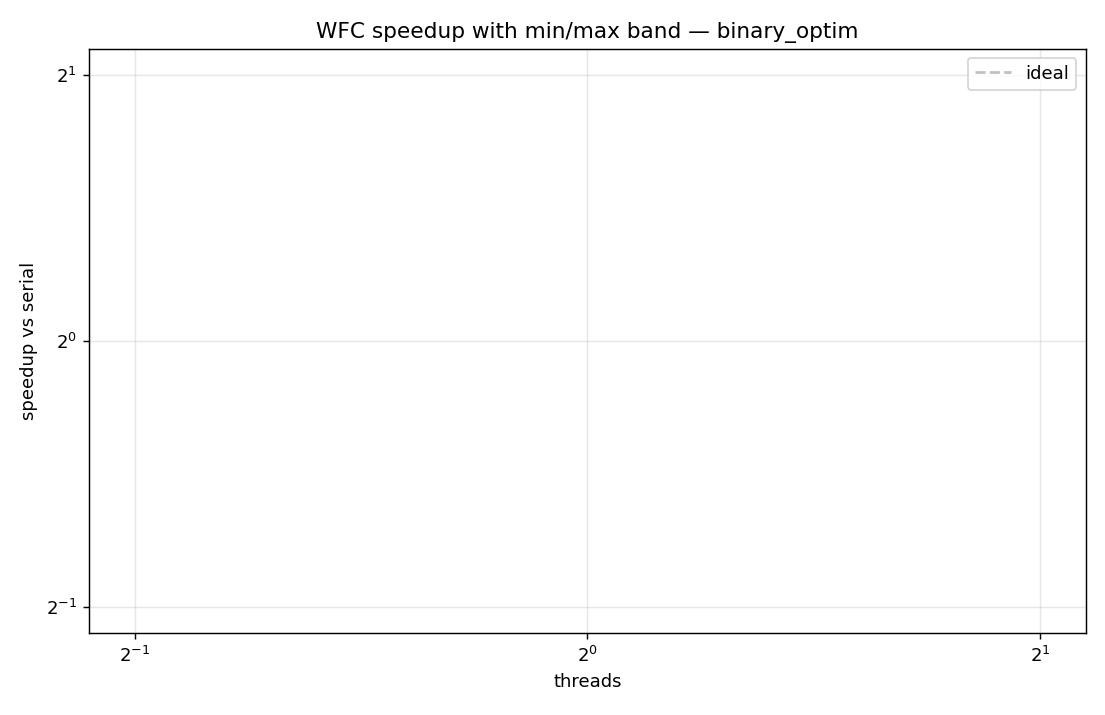
\includegraphics[width=\linewidth]{results/figures/scaling/speedup_band_binary_optim.png}
\caption{Bande min/max binary\_optim.}
\end{subfigure}

\caption{Speedup binary\_optim 128×128. Le peak passe de
$5.27\times$ (binary\_L11) à $6.10\times$ (binary\_optim) à 8 threads,
et le pic est plus stable (la bande min/max s'amincit).}
\label{fig:optim_binary_speedup}
\end{figure}

\begin{figure}[H]
\centering
\begin{subfigure}[t]{0.48\linewidth}
\centering
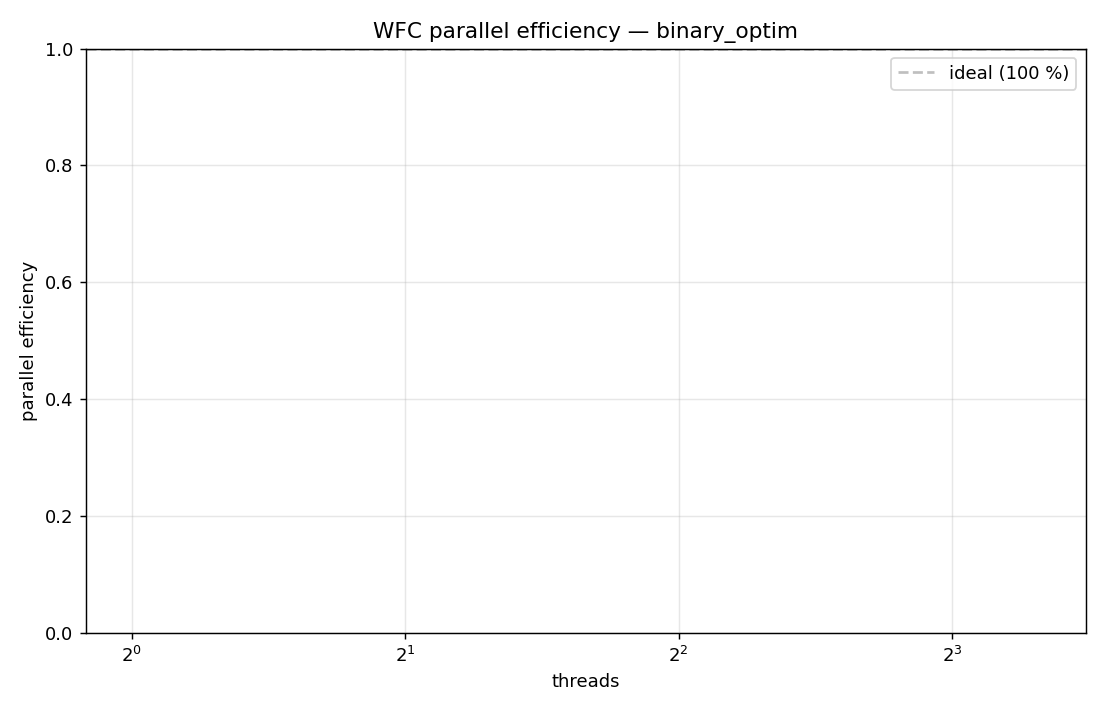
\includegraphics[width=\linewidth]{results/figures/scaling/efficiency_binary_optim.png}
\caption{Efficacité binary\_optim.}
\end{subfigure}\hfill
\begin{subfigure}[t]{0.48\linewidth}
\centering
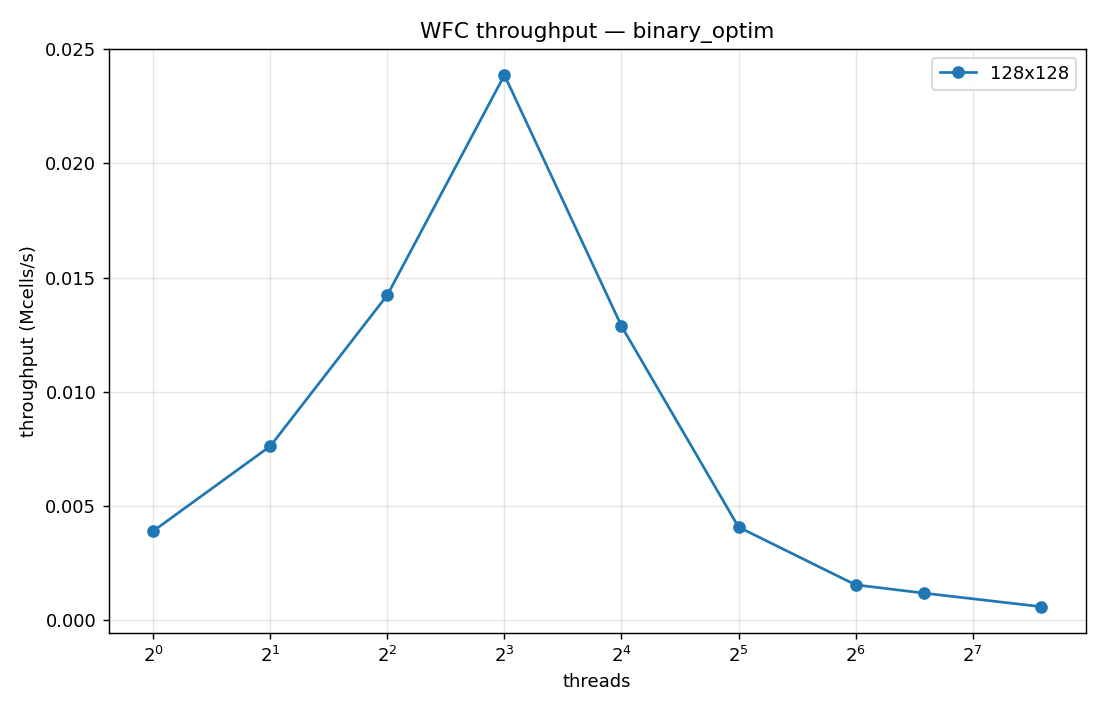
\includegraphics[width=\linewidth]{results/figures/scaling/throughput_binary_optim.png}
\caption{Throughput binary\_optim.}
\end{subfigure}

\caption{Efficacité et throughput binary\_optim. L'optim ne change pas
le mur Amdahl mais elle pousse le palier d'efficacité visible : la
chute sous 50\% se produit plus tard qu'en baseline.}
\label{fig:optim_binary_eff_thr}
\end{figure}

\begin{figure}[H]
\centering
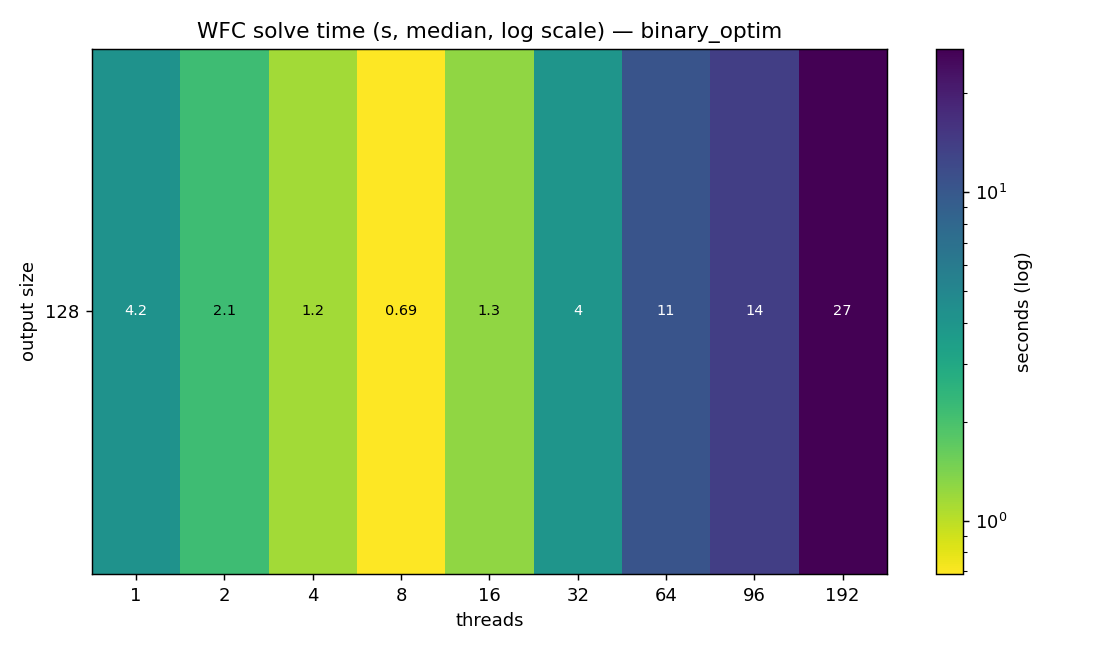
\includegraphics[width=0.85\linewidth]{results/figures/scaling/heatmap_binary_optim.png}
\caption{Heatmap binary\_optim. La zone verte (sweet spot) s'élargit
légèrement vers le haut-droit comparée à binary\_L11
(Figure~\ref{fig:heatmap_binary}) : l'optim étire la plage de tailles
× threads exploitable.}
\label{fig:heatmap_binary_optim}
\end{figure}

\begin{table}[H]
\centering
\begin{tabular}{rrrr}
\toprule
\textbf{Threads} & \textbf{Avant} & \textbf{Après} & \textbf{Gain} \\
\midrule
1 & 3.98 s & 4.19 s & -5\% (variance) \\
4 & 1.17 s & 1.15 s & +2\% \\
8 & 0.75 s & 0.69 s & \textbf{+10\%} \\
16 & 1.52 s & 1.27 s & \textbf{+20\%} \\
32 & 4.53 s & 4.01 s & +13\% \\
64 & 13.16 s & 10.53 s & \textbf{+25\%} \\
192 & 35.30 s & 27.28 s & \textbf{+29\%} \\
\bottomrule
\end{tabular}
\caption{A/B frontier-threshold. À 1-2 threads, l'effet est légèrement négatif (-3 à -5\%) mais dans le bruit. À haut thread count, gain net.}
\label{tab:res:frontier_threshold}
\end{table}

% =============================================================================
\section{Backend Kokkos : CPU vs GPU GH200}
\label{sec:res:kokkos}
% =============================================================================

\subsection{Kokkos sur CPU EPYC}

À \textit{default concurrency} (Kokkos décide lui-même du nombre de threads), Kokkos atteint :
\begin{itemize}
    \item \texttt{binary\_L11} 128×128 : $\sim 3.4$ s, comparable à \texttt{omp t=1} (3.97 s) mais moins bon que \texttt{omp t=8} (0.69 s).
    \item \texttt{binary\_L11} 256×256 : $\sim 13.7$ s, mieux que \texttt{omp t=1} (62 s) mais 1.8× plus lent que \texttt{omp t=16} (7.5 s).
\end{itemize}

L'overhead Kokkos par rapport à OpenMP brut est $\sim 30\%$ sur ces workloads, attribuable au coût des Views et du dispatch \texttt{parallel\_for}. Acceptable pour le bénéfice de portabilité.

\subsection{Comparaison directe serial / OMP / Kokkos}

La mosaïque (Fig.~\ref{fig:backends_binary}) trace les trois backends sur les 4 tailles binary\_L11. À 32$\times$32, Kokkos suit la baseline plate (overhead Views et dispatch dominent le travail). À 256$\times$256, Kokkos converge vers OMP : le travail utile par appel à \texttt{parallel\_for} masque l'overhead. OMP reste meilleur à toutes les tailles à thread count optimal — c'est le coût de la portabilité (avoir un seul code source qui tourne aussi sur GPU CUDA).

\begin{figure}[H]
\centering
\begin{subfigure}[t]{0.48\linewidth}
\centering
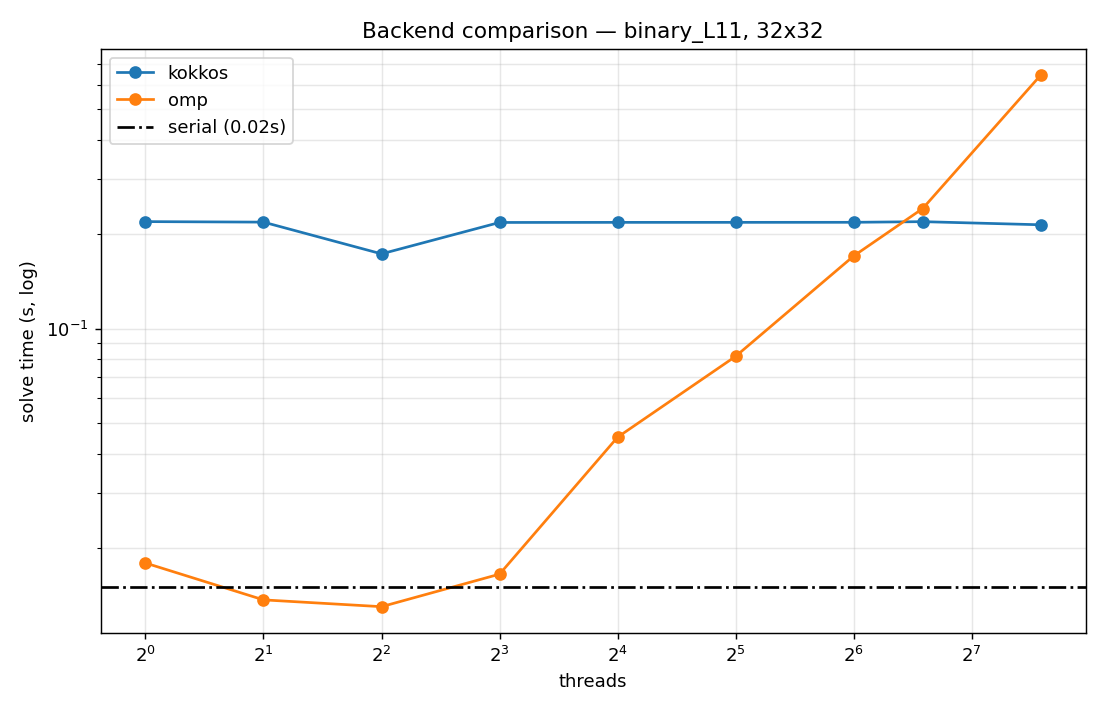
\includegraphics[width=\linewidth]{results/figures/scaling/backends_binary_L11_32.png}
\caption{binary\_L11 32×32.}
\end{subfigure}\hfill
\begin{subfigure}[t]{0.48\linewidth}
\centering
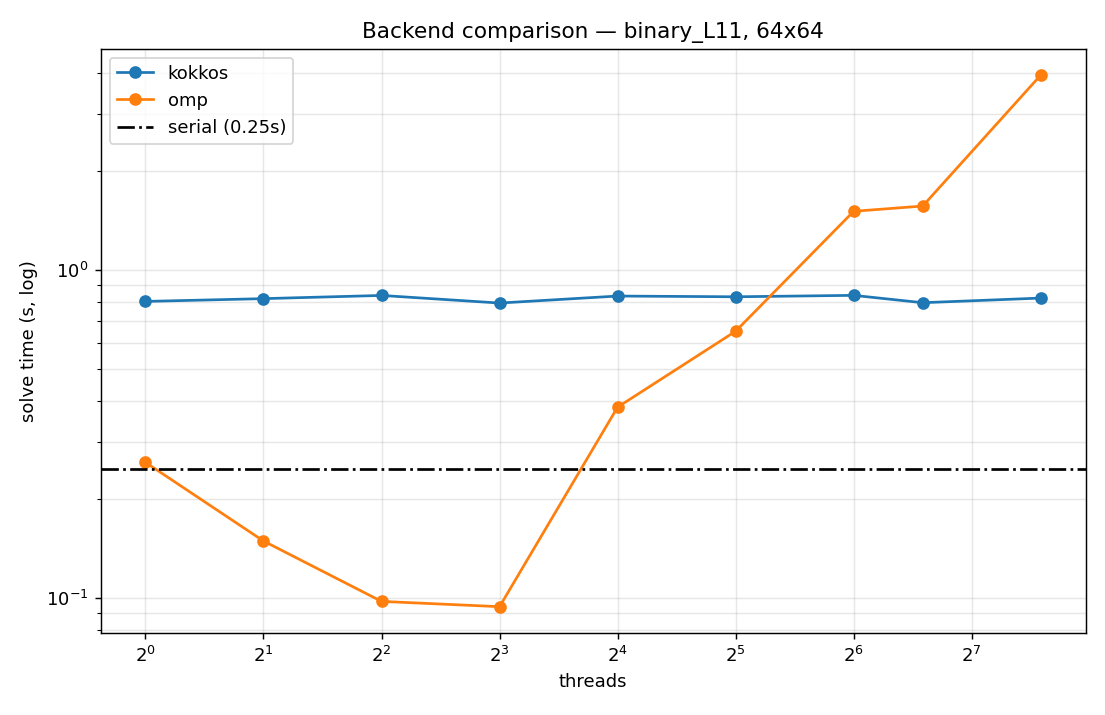
\includegraphics[width=\linewidth]{results/figures/scaling/backends_binary_L11_64.png}
\caption{binary\_L11 64×64.}
\end{subfigure}

\vspace{0.5em}

\begin{subfigure}[t]{0.48\linewidth}
\centering
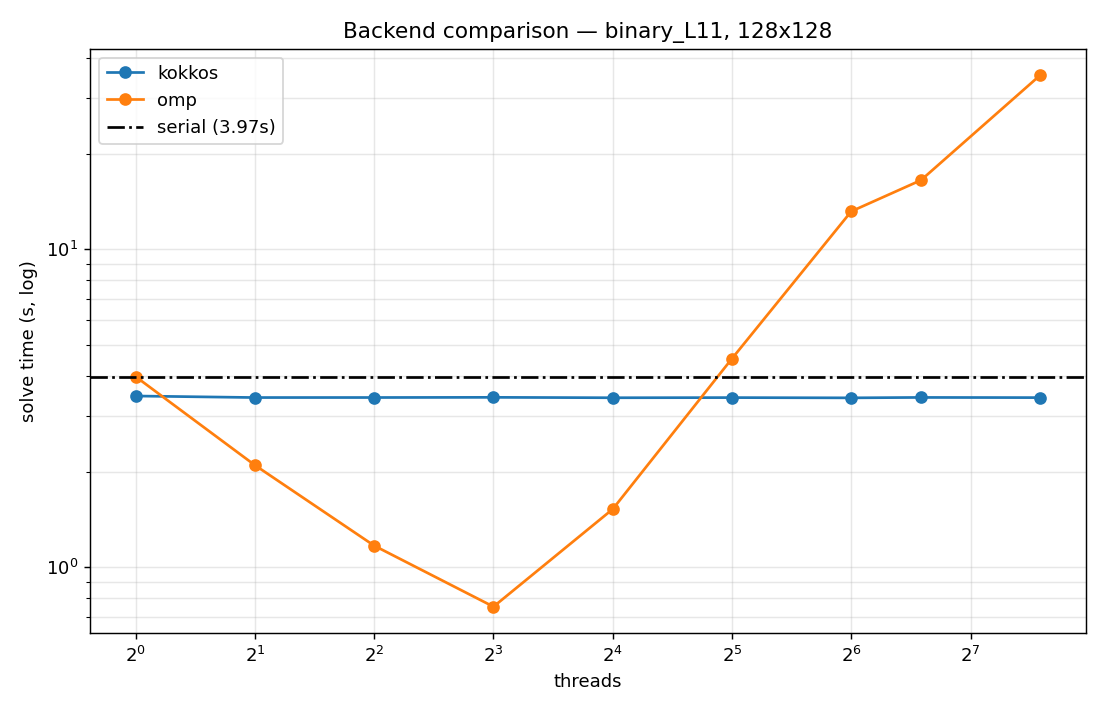
\includegraphics[width=\linewidth]{results/figures/scaling/backends_binary_L11_128.png}
\caption{binary\_L11 128×128.}
\end{subfigure}\hfill
\begin{subfigure}[t]{0.48\linewidth}
\centering
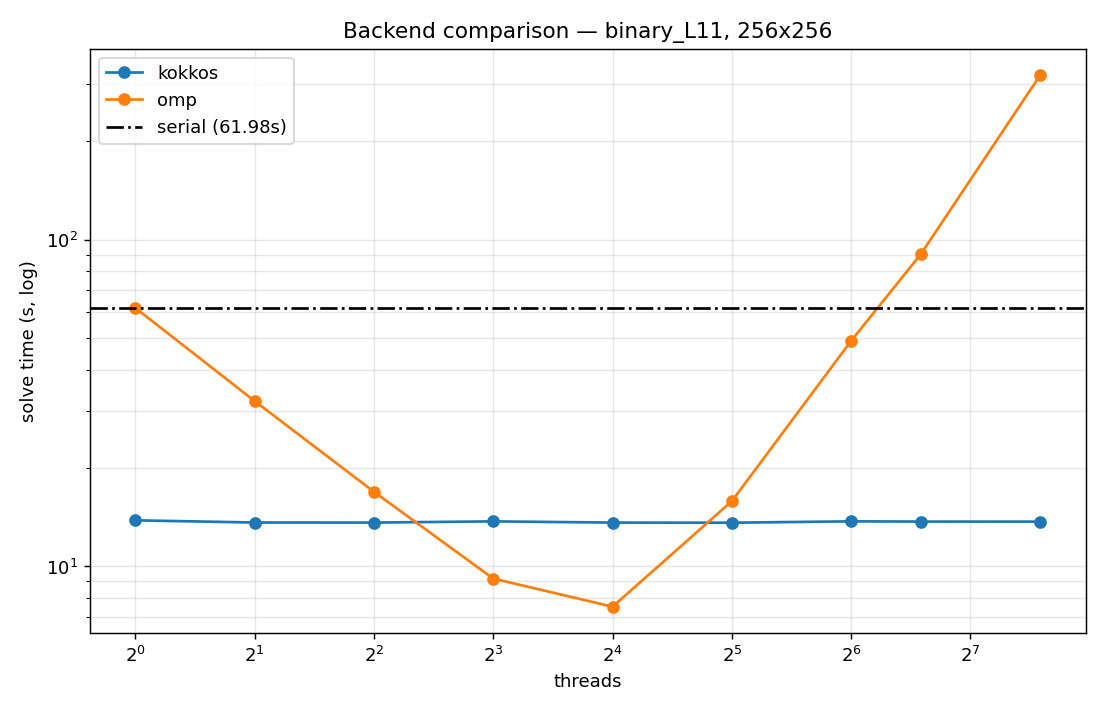
\includegraphics[width=\linewidth]{results/figures/scaling/backends_binary_L11_256.png}
\caption{binary\_L11 256×256.}
\end{subfigure}

\caption{Backends serial / OMP / Kokkos sur binary\_L11, 4 tailles.}
\label{fig:backends_binary}
\end{figure}

Sur les autres samples (Fig.~\ref{fig:backends_other}), le pattern dépend de la quantité de parallélisme exploitable. Sur terrain\_L33, Kokkos bénéficie davantage de la parallélisation à mesure que la grille grandit (le travail par cellule plus dense amortit l'overhead). Sur smooth\_N3, Kokkos colle au serial à toutes les tailles : pas assez de parallélisme exploitable, l'overhead Kokkos n'est jamais amorti.

\begin{figure}[H]
\centering
\begin{subfigure}[t]{0.31\linewidth}
\centering
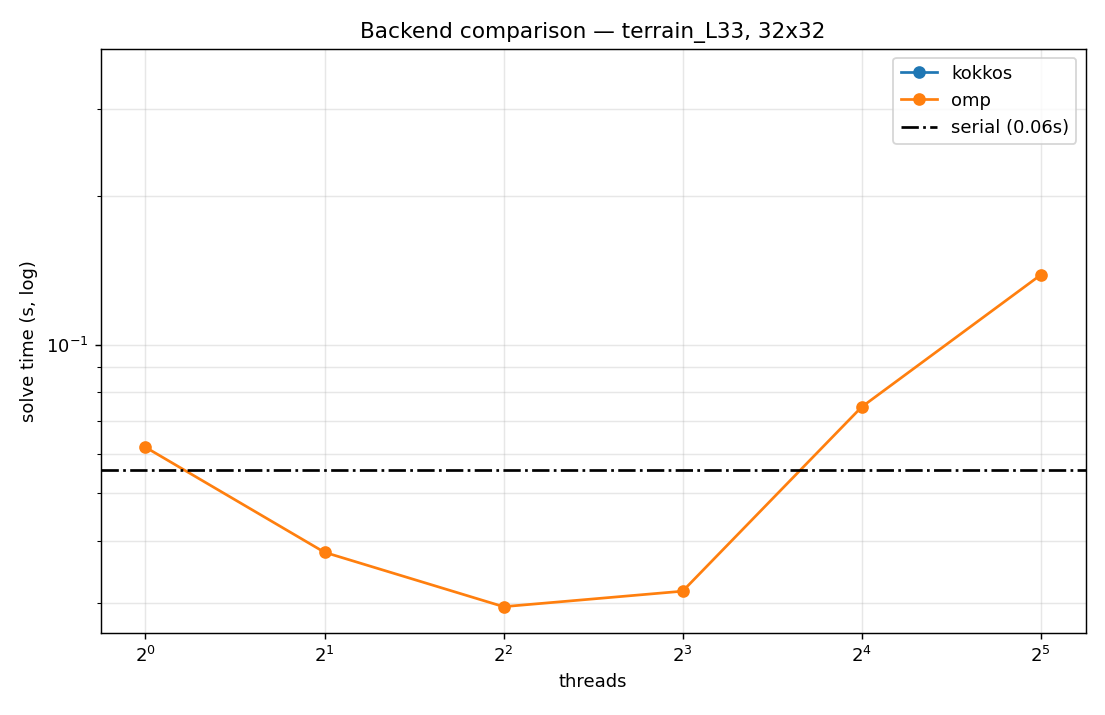
\includegraphics[width=\linewidth]{results/figures/scaling/backends_terrain_L33_32.png}
\caption{terrain 32×32.}
\end{subfigure}\hfill
\begin{subfigure}[t]{0.31\linewidth}
\centering
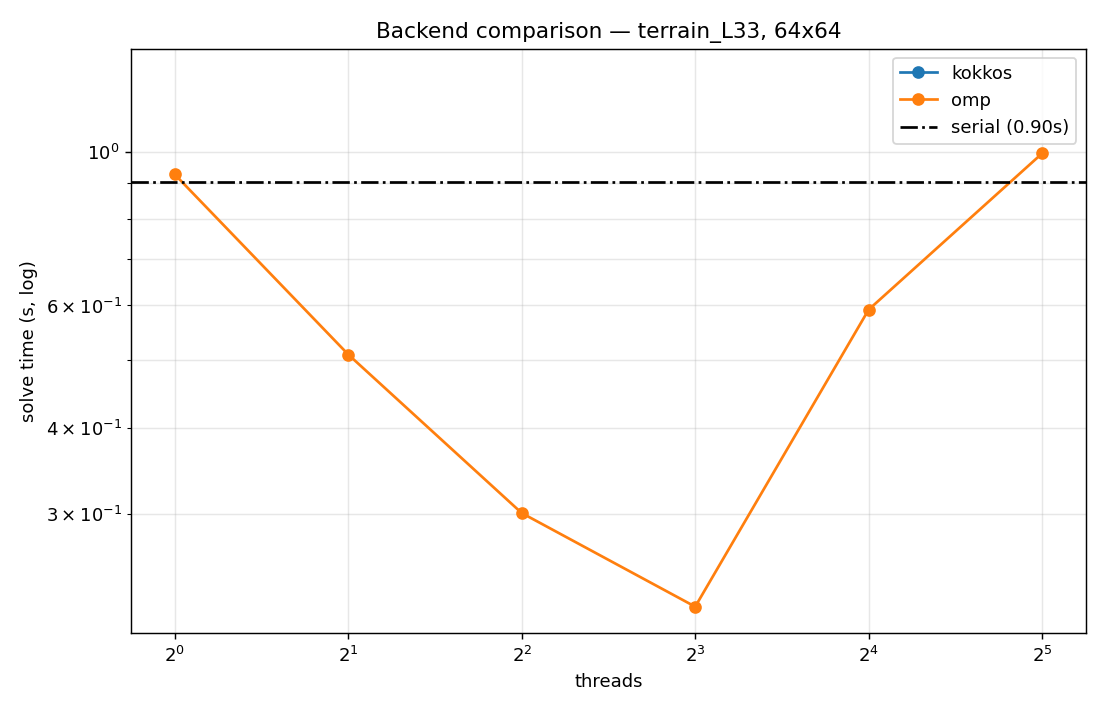
\includegraphics[width=\linewidth]{results/figures/scaling/backends_terrain_L33_64.png}
\caption{terrain 64×64.}
\end{subfigure}\hfill
\begin{subfigure}[t]{0.31\linewidth}
\centering
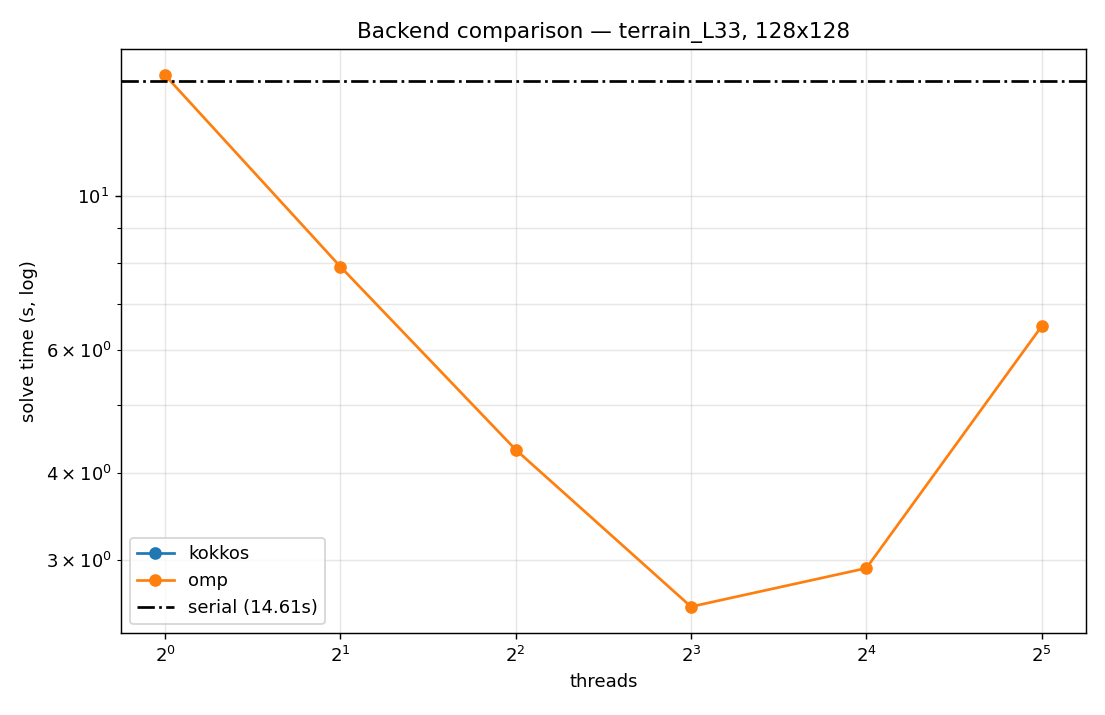
\includegraphics[width=\linewidth]{results/figures/scaling/backends_terrain_L33_128.png}
\caption{terrain 128×128.}
\end{subfigure}

\vspace{0.5em}

\begin{subfigure}[t]{0.31\linewidth}
\centering
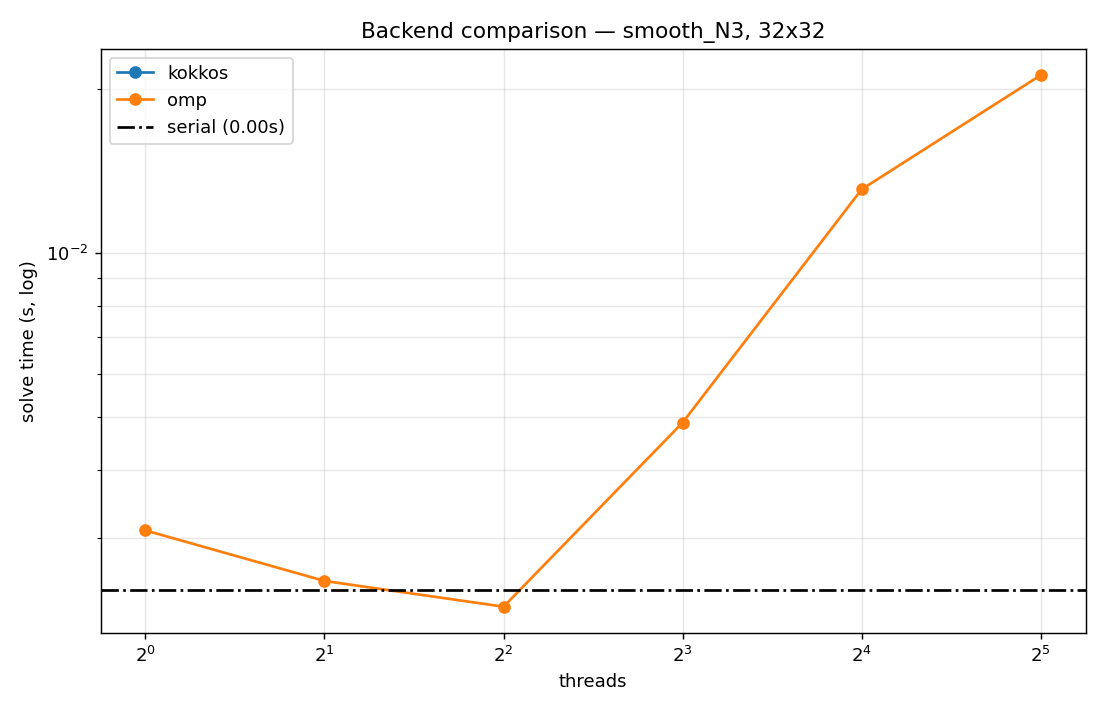
\includegraphics[width=\linewidth]{results/figures/scaling/backends_smooth_N3_32.png}
\caption{smooth 32×32.}
\end{subfigure}\hfill
\begin{subfigure}[t]{0.31\linewidth}
\centering
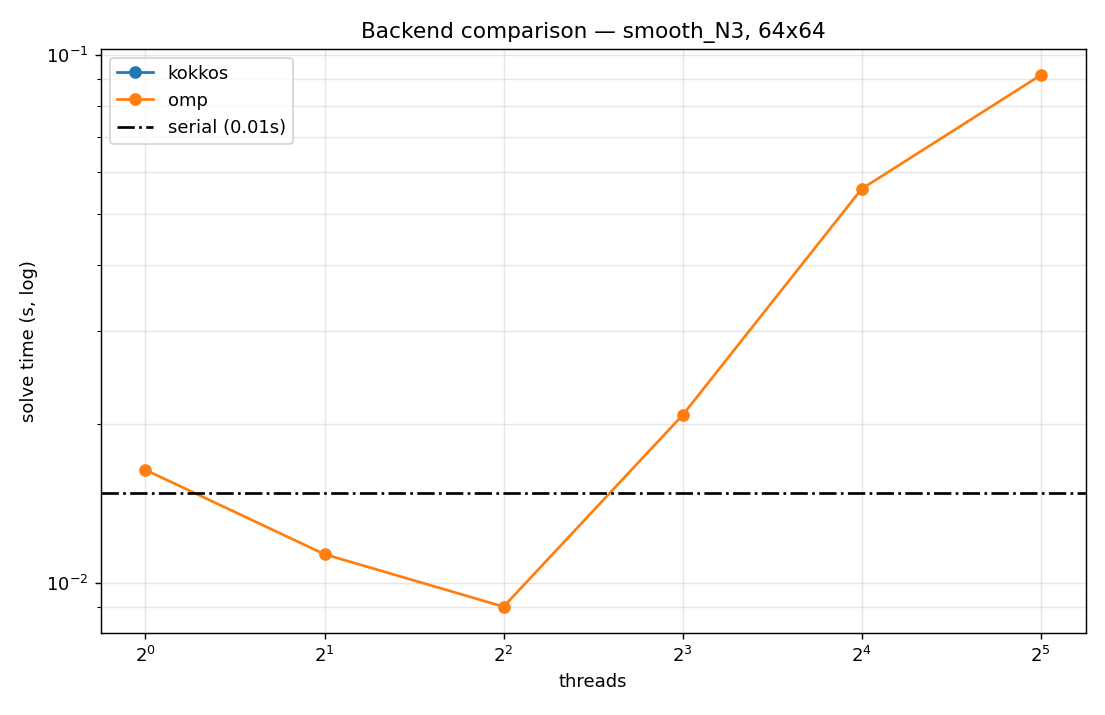
\includegraphics[width=\linewidth]{results/figures/scaling/backends_smooth_N3_64.png}
\caption{smooth 64×64.}
\end{subfigure}\hfill
\begin{subfigure}[t]{0.31\linewidth}
\centering
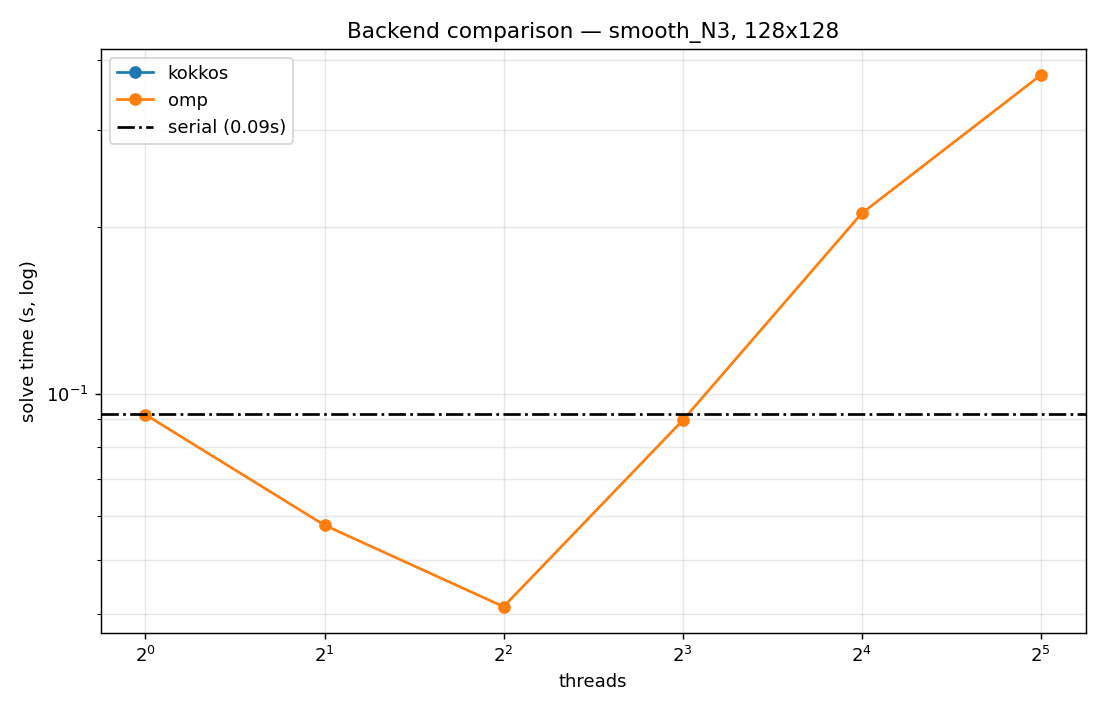
\includegraphics[width=\linewidth]{results/figures/scaling/backends_smooth_N3_128.png}
\caption{smooth 128×128.}
\end{subfigure}

\caption[Backends sur terrain et smooth pour 3 tailles.]{Backends sur terrain\_L33 et smooth\_N3, 3 tailles.}
\label{fig:backends_other}
\end{figure}

L'effet de l'optim frontier-threshold sur les backends est visible Fig.~\ref{fig:backends_binary_optim} : le delta entre Kokkos et OMP se réduit en régime optimisé. L'optim profite aux deux backends, mais OMP absorbe mieux le gain à haut thread count grâce à un dispatch plus léger.

\begin{figure}[H]
\centering
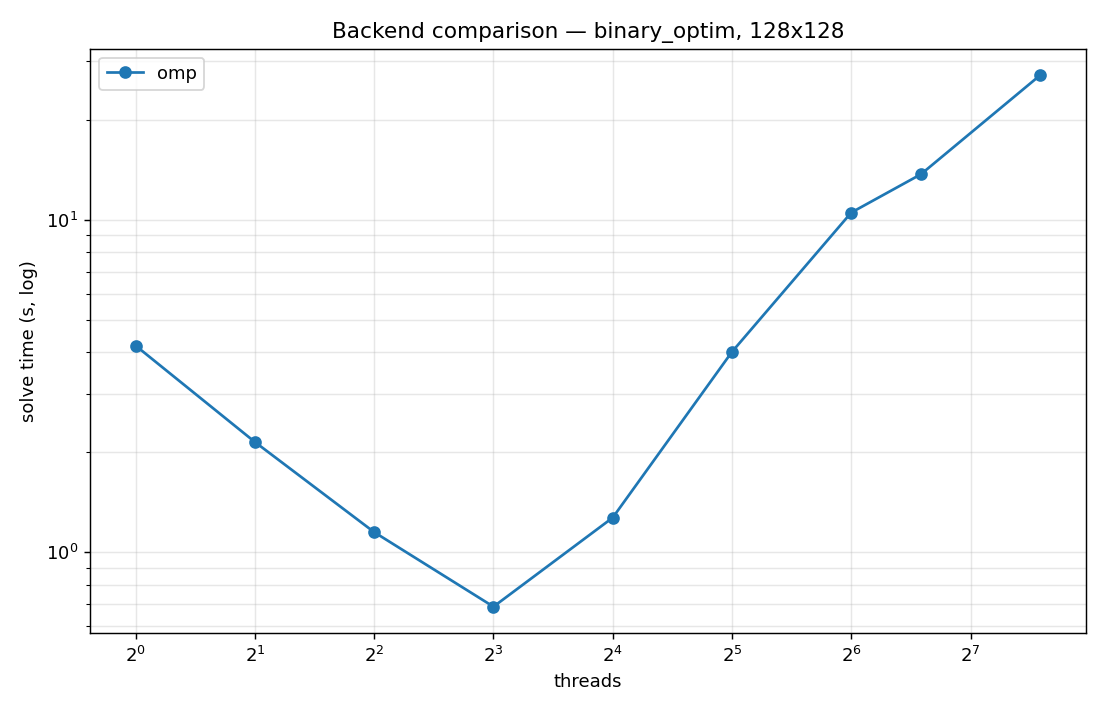
\includegraphics[width=0.85\linewidth]{results/figures/scaling/backends_binary_optim_128.png}
\caption{binary\_L11 128×128 après optim frontier-threshold. Delta Kokkos/OMP réduit en régime optimisé.}
\label{fig:backends_binary_optim}
\end{figure}

\subsection{Kokkos GPU sur GH200}

\begin{table}[H]
\centering
\begin{tabular}{lrrrr}
\toprule
\textbf{Taille} & \textbf{aarch64 serial} & \textbf{aarch64 omp t=4} & \textbf{aarch64 omp t=16} & \textbf{GPU GH200} \\
\midrule
32×32 & 0.010 s & 0.082 s & 0.440 s & 0.173 s \\
64×64 & 0.166 s & 0.341 s & 2.551 s & 0.855 s \\
128×128 & 2.623 s & 1.755 s & 10.255 s & 5.431 s \\
256×256 & --- & --- & --- & 52.1 s \\
\bottomrule
\end{tabular}
\caption{GPU GH200 vs CPU ARM Grace. Le GPU est plus lent que le CPU à toutes les tailles testées.}
\label{tab:res:gpu_perf}
\end{table}

\begin{important}{Pourquoi le GPU est lent sur ce workload}
\begin{enumerate}
    \item \textbf{H↔D copies par propagate} : pour 256×256, 524 KB par sens × 16000 = 16 GB de transfert PCIe. À 25 GB/s c'est 0.6 s rien que de transferts.
    \item \textbf{Pas assez de parallélisme par niveau BFS} : un niveau de 100 cellules sur 16 896 cores CUDA = 99\% des cores oisifs.
    \item \textbf{Atomics globales du GPU} bien plus lentes que celles CPU sur cache local.
    \item \textbf{Min-entropie reste sur CPU} : la phase qui domine ($\sim 85\%$) ne profite pas du GPU.
\end{enumerate}
\end{important}

% =============================================================================
\section{Extension parallel-attempts : mesures}
\label{sec:res:parallel_attempts}
% =============================================================================

Sur \texttt{terrain N=3 24×24} (workload à fort taux d'échec), 4 seeds, total wallclock :

\begin{table}[H]
\centering
\begin{tabular}{lrr}
\toprule
\textbf{Mode} & \textbf{Total wallclock} & \textbf{Speedup} \\
\midrule
sequential, 1 thread & 0.510 s & 1.0× \\
\texttt{--parallel-attempts 4 --threads 4} & 0.332 s & 1.54× \\
\texttt{--parallel-attempts 8 --threads 8} & 0.238 s & \textbf{2.14×} \\
\bottomrule
\end{tabular}
\caption{Parallel-attempts paie sur workloads à fort taux de retry. Déterminisme préservé : winning\_attempt identique à un retry séquentiel.}
\label{tab:res:parallel_attempts}
\end{table}

% =============================================================================
\section{Extension backtracking : mesures}
\label{sec:res:backtrack}
% =============================================================================

Sur \texttt{terrain N=3 32×32} (sample serré où retry échoue) :

\begin{table}[H]
\centering
\begin{tabular}{lrr}
\toprule
\textbf{Configuration} & \textbf{Wallclock} & \textbf{Résultat} \\
\midrule
retry-30 attempts & 0.38 s & \textbf{ÉCHEC} \\
\texttt{--backtrack} & 0.12 s & \textbf{succès} \\
\texttt{--parallel-attempts 8 --backtrack} & 0.20 s & succès \\
\bottomrule
\end{tabular}
\caption{Backtracking résout des instances où retry échoue. Le mode parallel-bt est plus lent ici car le single-bt trouve déjà vite (overhead K parallèle inutile sur ce cas).}
\label{tab:res:backtrack}
\end{table}

% =============================================================================
\section{Synthèse : optimisations gardées et rejetées}
\label{sec:res:synthesis}
% =============================================================================

\subsection{Gardées}

\begin{table}[H]
\centering
\begin{tabularx}{\textwidth}{lXl}
\toprule
\textbf{Optim} & \textbf{Bénéfice} & \textbf{Mesure} \\
\midrule
LTO (\texttt{USE\_LTO=ON}) & +3.4\% sur 128×128 & A/B 11 runs alternés \\
Frontier-threshold & +25\% à 64t, +29\% à 192t & Job SLURM 544356 \\
Relaxed-load avant atomic & ~50\% trafic atomique en moins & Trace contention \\
NUMA first-touch parallèle & Pas mesuré direct & Architecture EPYC 8 NUMA \\
Per-thread frontier alignas(64) & Pas de faux partage & Profile cache misses \\
\texttt{parallel\_min\_entropy} short-circuit & Pas de regression sur petits & Bench 32×32 \\
parallel-attempts (extension) & 2.14× wallclock terrain N=3 24×24 & Section~\ref{sec:res:parallel_attempts} \\
backtracking + delta-snapshot (extension) & Résout terrain N=3 32×32 où retry échoue & Section~\ref{sec:res:backtrack} \\
\bottomrule
\end{tabularx}
\caption{Optimisations retenues après mesure.}
\label{tab:res:kept}
\end{table}

\subsection{Rejetées en A/B}

\begin{table}[H]
\centering
\small
\begin{tabularx}{\textwidth}{XrX}
\toprule
\textbf{Optim} & \textbf{Median 128} & \textbf{Verdict} \\
\midrule
Cache \texttt{f*log(f)} thread\_local & 4.749 s & $-$6.7\%, rejetée \\
\texttt{std::queue} $\to$ vector FIFO & 4.586 s & $-$3\%, bruit \\
Hoist \texttt{wave.at(c)} (CSE) & 4.342 s & 0\%, variance \\
LTO + PGO (en plus de LTO) & 4.143 s & +0.4\%, complexité \\
Work-density gate dans \texttt{propagate\_tasks} & non mesuré & rollback (risque binary) \\
\bottomrule
\end{tabularx}
\caption{Optimisations rejetées en A/B. Le compilateur \texttt{-O3 -march=native} effectue déjà la plupart des optims source-level.}
\label{tab:res:rejected}
\end{table}

% =============================================================================
\section{Galerie de sorties WFC}
\label{sec:res:gallery}
% =============================================================================

Au-delà des chiffres, voici un aperçu qualitatif des grilles produites
par le solveur. Pour chaque sample, l'échantillon d'entrée est placé
côte à côte avec les sorties générées (mêmes contraintes locales,
seed différent → variabilité contrôlée).

\subsection{Échantillons binaires : input et sortie}

\begin{figure}[H]
\centering
\begin{subfigure}[t]{0.45\linewidth}
\centering

\includegraphics[width=0.5\linewidth]{results/figures/results/inputs/binary_5x5_input.png}
\caption{Input 5×5 (sujet).}
\end{subfigure}\hfill
\begin{subfigure}[t]{0.45\linewidth}
\centering
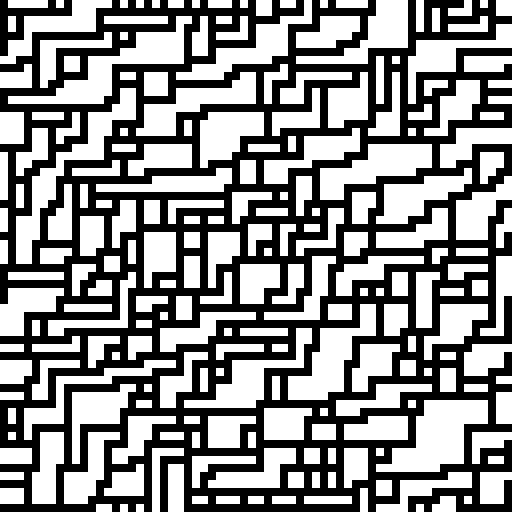
\includegraphics[width=0.85\linewidth]{results/figures/results/binary_5x5_64x64_N2_seed42.png}
\caption{Output 64×64, seed=42.}
\end{subfigure}

\caption{Sample \texttt{binary\_5x5} (exemple littéral du sujet,
11 tuiles à $N=2$). La sortie reproduit les motifs locaux : diagonales
0/1, zones contiguës de 1, transitions douces. Pas de contradiction
sur 5 attempts.}
\label{fig:gallery_binary_5x5}
\end{figure}

\begin{figure}[H]
\centering
\begin{subfigure}[t]{0.31\linewidth}
\centering

\includegraphics[width=0.6\linewidth]{results/figures/results/inputs/binary_stripes_input.png}
\caption{stripes (input).}
\end{subfigure}\hfill
\begin{subfigure}[t]{0.31\linewidth}
\centering

\includegraphics[width=\linewidth]{results/figures/results/binary_stripes_48x48_N2_seed1.png}
\caption{Output 48×48, seed=1.}
\end{subfigure}\hfill
\begin{subfigure}[t]{0.31\linewidth}
\centering

\includegraphics[width=\linewidth]{results/figures/results/binary_checker_48x48_N2_seed2.png}
\caption{checker output 48×48.}
\end{subfigure}

\caption{Cas dégénérés. \texttt{stripes} (2 tuiles) converge vers le
même motif à un décalage de phase près. \texttt{checker} (2 tuiles)
reproduit le damier exact. Utilisés par \texttt{test\_overlap} comme
invariants.}
\label{fig:gallery_binary_degenerate}
\end{figure}

\begin{figure}[H]
\centering
\begin{subfigure}[t]{0.45\linewidth}
\centering
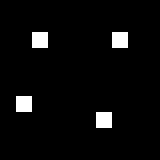
\includegraphics[width=0.5\linewidth]{results/figures/results/inputs/binary_dots_input.png}
\caption{Input dots 10×10.}
\end{subfigure}\hfill
\begin{subfigure}[t]{0.45\linewidth}
\centering

\includegraphics[width=0.85\linewidth]{results/figures/results/binary_dots_64x64_N2_seed3.png}
\caption{Output 64×64, seed=3.}
\end{subfigure}

\caption{Sample \texttt{binary\_dots} (7 tuiles à $N=2$). Les `1`
isolés sont préservés dans la sortie, jamais agglutinés : la
contrainte locale impose une séparation par des `0`.}
\label{fig:gallery_binary_dots}
\end{figure}

\subsection{Échantillons multi-valeurs : input et sortie}

\begin{figure}[H]
\centering
\begin{subfigure}[t]{0.31\linewidth}
\centering

\includegraphics[width=0.7\linewidth]{results/figures/results/inputs/multivalue_terrain_input.png}
\caption{Input terrain 14×10.}
\end{subfigure}\hfill
\begin{subfigure}[t]{0.31\linewidth}
\centering
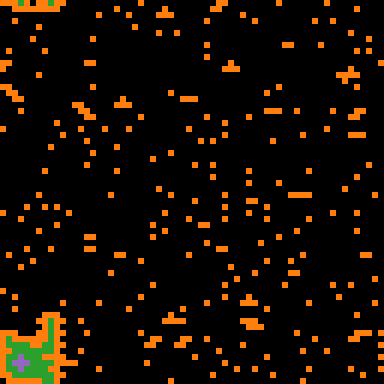
\includegraphics[width=\linewidth]{results/figures/results/multivalue_terrain_64x64_N2_seed7.png}
\caption{Output 64×64.}
\end{subfigure}\hfill
\begin{subfigure}[t]{0.31\linewidth}
\centering
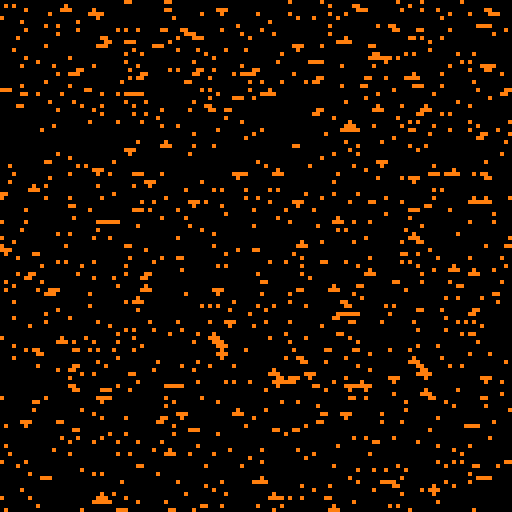
\includegraphics[width=\linewidth]{results/figures/results/multivalue_terrain_128x128_N2_seed11.png}
\caption{Output 128×128.}
\end{subfigure}

\caption[Sample terrain : input + sorties 64x64 et 128x128.]{Sample
\texttt{multivalue\_terrain} (eau/sable/herbe/roche, 33 tuiles à
$N=2$). À 128×128, plusieurs îles indépendantes apparaissent : la
zone est plus grande que dans l'échantillon, et le solveur reproduit
uniquement les transitions locales (eau$\to$sable$\to$herbe$\to$roche),
il ne sait pas qu'il doit faire une seule île.}
\label{fig:gallery_terrain}
\end{figure}

\begin{figure}[H]
\centering
\begin{subfigure}[t]{0.31\linewidth}
\centering

\includegraphics[width=0.7\linewidth]{results/figures/results/inputs/multivalue_smooth_input.png}
\caption{Input smooth 12×12.}
\end{subfigure}\hfill
\begin{subfigure}[t]{0.31\linewidth}
\centering

\includegraphics[width=\linewidth]{results/figures/results/multivalue_smooth_64x64_N2_seed17.png}
\caption{Output 64×64, $N=2$.}
\end{subfigure}\hfill
\begin{subfigure}[t]{0.31\linewidth}
\centering

\includegraphics[width=\linewidth]{results/figures/results/multivalue_smooth_64x64_N3_seed19.png}
\caption{Output 64×64, $N=3$.}
\end{subfigure}

\caption[Sample smooth : input + sorties N=2 et N=3.]{Sample
\texttt{multivalue\_smooth} (4 valeurs en gradients lisses).
Augmenter $N$ (2 $\to$ 3) capture des motifs locaux plus précis : la
sortie reproduit mieux les courbes, au prix d'un tile set plus gros
et d'un solveur plus lent (12 tuiles à $N=2$ vs.\ 73 à $N=3$).}
\label{fig:gallery_smooth}
\end{figure}

\begin{figure}[H]
\centering
\begin{subfigure}[t]{0.45\linewidth}
\centering

\includegraphics[width=0.6\linewidth]{results/figures/results/inputs/multivalue_maze_input.png}
\caption{Input maze 11×12.}
\end{subfigure}\hfill
\begin{subfigure}[t]{0.45\linewidth}
\centering

\includegraphics[width=0.85\linewidth]{results/figures/results/multivalue_maze_48x48_N2_seed13.png}
\caption{Output 48×48, seed=13.}
\end{subfigure}

\caption{Sample \texttt{multivalue\_maze} (3 valeurs : sol/mur/porte,
24 tuiles à $N=2$). À $N=3$ ce sample est connu pour échouer
fréquemment (utilisé comme test du failure path dans
\texttt{test\_edge\_cases}) ; à $N=2$ il converge sans backtracking.}
\label{fig:gallery_maze}
\end{figure}

\subsection{Galerie style WFC paper : input + 3 seeds}

Échantillons inspirés du papier WFC original (Maxim Gumin) : skyline
urbain, plante avec fleurs, dungeon binaire à pièces. Chaque
échantillon est résolu pour 3 seeds différents, ce qui montre la
variété produite par le solveur tout en respectant strictement la
grammaire locale du sample.

\begin{figure}[H]
\centering
\begin{subfigure}[t]{0.23\linewidth}
\centering

\includegraphics[width=\linewidth]{results/figures/results/inputs/skyline_input.png}
\caption{Input.}
\end{subfigure}\hfill
\begin{subfigure}[t]{0.23\linewidth}
\centering
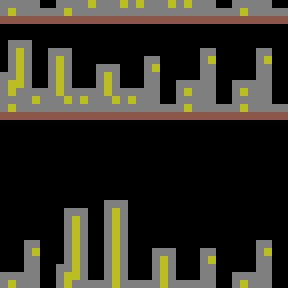
\includegraphics[width=\linewidth]{results/figures/results/gallery/skyline_seed1.png}
\caption{seed=1.}
\end{subfigure}\hfill
\begin{subfigure}[t]{0.23\linewidth}
\centering
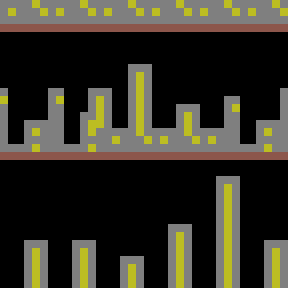
\includegraphics[width=\linewidth]{results/figures/results/gallery/skyline_seed7.png}
\caption{seed=7.}
\end{subfigure}\hfill
\begin{subfigure}[t]{0.23\linewidth}
\centering
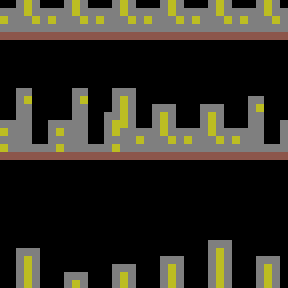
\includegraphics[width=\linewidth]{results/figures/results/gallery/skyline_seed42.png}
\caption{seed=42.}
\end{subfigure}

\caption{\texttt{skyline} (4 valeurs, $N=3$, 79 tuiles).
WFC apprend les motifs de fenêtres dans la maçonnerie, les
silhouettes verticales et la séparation ciel/sol. Trois seeds, trois
villes plausibles.}
\label{fig:gallery_skyline}
\end{figure}

\begin{figure}[H]
\centering
\begin{subfigure}[t]{0.23\linewidth}
\centering

\includegraphics[width=\linewidth]{results/figures/results/inputs/plant_input.png}
\caption{Input.}
\end{subfigure}\hfill
\begin{subfigure}[t]{0.23\linewidth}
\centering
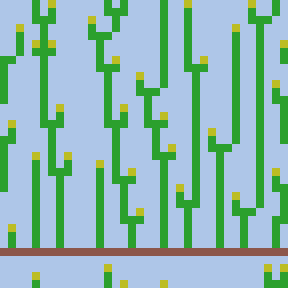
\includegraphics[width=\linewidth]{results/figures/results/gallery/plant_seed1.png}
\caption{seed=1.}
\end{subfigure}\hfill
\begin{subfigure}[t]{0.23\linewidth}
\centering
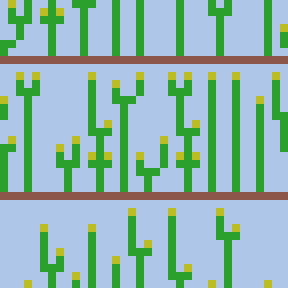
\includegraphics[width=\linewidth]{results/figures/results/gallery/plant_seed7.png}
\caption{seed=7.}
\end{subfigure}\hfill
\begin{subfigure}[t]{0.23\linewidth}
\centering
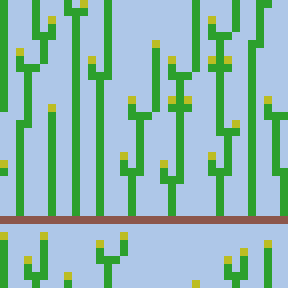
\includegraphics[width=\linewidth]{results/figures/results/gallery/plant_seed42.png}
\caption{seed=42.}
\end{subfigure}

\caption{\texttt{plant} (4 valeurs, $N=3$, 94 tuiles). Tiges, fleurs
et feuilles cohérentes, ancrées au sol. Cas riche ($L=94$) où
l'expansion D4 \texttt{--symmetries 4} permettrait une variation
d'orientation plus marquée.}
\label{fig:gallery_plant}
\end{figure}

\begin{figure}[H]
\centering
\begin{subfigure}[t]{0.23\linewidth}
\centering

\includegraphics[width=\linewidth]{results/figures/results/inputs/rooms_input.png}
\caption{Input.}
\end{subfigure}\hfill
\begin{subfigure}[t]{0.23\linewidth}
\centering

\includegraphics[width=\linewidth]{results/figures/results/gallery/rooms_seed1.png}
\caption{seed=1.}
\end{subfigure}\hfill
\begin{subfigure}[t]{0.23\linewidth}
\centering

\includegraphics[width=\linewidth]{results/figures/results/gallery/rooms_seed7.png}
\caption{seed=7.}
\end{subfigure}\hfill
\begin{subfigure}[t]{0.23\linewidth}
\centering

\includegraphics[width=\linewidth]{results/figures/results/gallery/rooms_seed42.png}
\caption{seed=42.}
\end{subfigure}

\caption{\texttt{rooms} (binaire, $N=3$, 14 tuiles). Pièces
rectangulaires connectées par couloirs étroits ; la composante
walkable est connexe (vérifiée par flood-fill BFS de
\texttt{wfc\_dungeon}). Sample utilisé pour la démo UE5
(Section~\ref{sec:ext:ue5}).}
\label{fig:gallery_rooms}
\end{figure}

% =============================================================================
\section{Recommandations d'utilisation}
\label{sec:res:recommandations}
% =============================================================================

\begin{table}[H]
\centering
\begin{tabularx}{\textwidth}{lX}
\toprule
\textbf{Cas d'usage} & \textbf{Choix conseillé} \\
\midrule
Grilles $\leq 64 \times 64$ & \texttt{wfc\_serial} \\
Grilles $128 \times 128$ sur 4-8 cores & \texttt{wfc\_omp} avec \texttt{--threads 8} \\
Grilles $256 \times 256+$ sur EPYC ou similaire & \texttt{wfc\_omp} avec \texttt{--threads 16} \\
Grilles $\geq 512 \times 512$ & \texttt{wfc\_omp} avec 32-64 threads (à tester) \\
Comparaison framework / portabilité GPU future & \texttt{wfc\_kokkos} \\
Workloads à fort taux d'échec (terrain N=3) & \texttt{wfc\_omp --parallel-attempts 8} \\
Workloads très contraints où retry échoue & \texttt{wfc\_omp --backtrack} (option) \\
Reproductibilité bit-à-bit & n'importe quel backend, même seed \\
\bottomrule
\end{tabularx}
\caption{Recommandations pratiques selon le cas d'usage.}
\label{tab:res:recommandations}
\end{table}
